\documentclass{midl}

\usepackage{amsmath,amssymb,amsfonts}
\usepackage{graphicx}
\usepackage{booktabs}
\usepackage{array}
\usepackage{textcomp}
\usepackage{xcolor}
\usepackage{url}
\usepackage{tikz}
\usepackage{pgfplots}
\pgfplotsset{compat=1.18}
\usetikzlibrary{arrows.meta,positioning,calc,shapes.geometric}
\def\figureautorefname{Figure}
\def\tableautorefname{Table}
\def\equationautorefname{Equation}

\jmlrvolume{-- Under Review}
\jmlryear{2027}
\jmlrworkshop{Full Paper -- MIDL 2027 submission}
\editors{Under Review for MIDL 2027}

\newcommand{\SOtwo}{\mathrm{SO}(2)}

\title[Rotation-Equivariant VAEs for Histopathology]{Rotation-Equivariant Variational Autoencoders for Representation
Learning and Downstream Classification in Histopathology}

\midlauthor{\Name{Maximiliano Garavito Chtefan} \Email{maximiliano2162094@correo.uis.edu.co}\\
\Name{David Romo-Bucheli} \Email{deromob@uis.edu.co}\\
\addr Escuela de Ingenier\'ia de Sistemas e Inform\'atica\\
Universidad Industrial de Santander, Bucaramanga, Colombia
}

\begin{document}

\maketitle

\begin{abstract}
At high magnification, cellular patterns in histopathology have no dominant orientation in the image, making rotation a relevant local symmetry for representation learning. This work investigates whether incorporating this rotation symmetry into unsupervised representation learning improves reconstruction and performance in downstream classification tasks. We first train a conventional denoising variational autoencoder (VAE) and a continuous-$\SOtwo$-equivariant denoising VAE trained on the same unlabeled patches from ovarian cancer images. With both autoencoders models' weights frozen, reconstruction was evaluated on patches from held-out whole-slide images (WSIs). Afterwards, we evaluated the representation capability of both autoencoders in two downstream tasks: three-class tissue recognition at patch level, and five-class WSI diagnosis via multiple-instance learning. Reconstruction mean absolute error for the test patches was $0.0629$ versus $0.0642$ (conventional versus equivariant), but the difference was not statistically significant. For three-class tissue recognition with a small budget of 500 training labels per class, the equivariant VAE outperforms the conventional VAE with a macro-F1 of $0.511$ versus $0.575$. For other budgets tested (250, 1000, 2500 and 5671) no statistical difference was found, although the equivariant VAE perfomed better in all the budgets except for the largest one. For WSI diagnosis, five-fold cross-validation uses the 361-slide VAE-development cohort. Final classifiers are trained on all 361 development WSIs and evaluated on a separate cohort of 152 WSIs, with macro-F1 values of $XXXX$ versus $YYYY$ (conventional versus equivariant).
% TODO: Completar XXXX/YYYY y la interpretacion estadistica con la evaluacion MIL final de las 152 WSIs.
\end{abstract}

\begin{keywords}
histopathology, variational autoencoder, rotation equivariance, $\SOtwo$, whole-slide image classification, representation learning
\end{keywords}

\section{Introduction}

Digital histopathology allows for digitization of glass slides into whole-slide images whose dimensions commonly reach gigapixel scale. These images contain many local tissue regions, but their diagnostic labels and detailed annotations require specialist review. Representation learning via unlabeled patches allows machine learning models to extract useful representations for using in a downstream task.~\cite{litjens_survey_2017,song_artificial_2023,tellez_neural_2021}.

While orientation can be relevant to tissue architecture at lower magnification, cellular patterns at high magnification have no dominant orientation in the image. At this scale, a rotation changes the viewing orientation of a patch while preserving its tissue identity and diagnostic information. This rotational symmetry motivates incorporating rotation into the model's architectural constraints. Ordinary convolutional neural networks (CNNs) use convolutions that are equivariant to translations: translating an input translates its computed feature map~\cite{lecun_gradient_1998,cohen_group_2016}. Conventional CNNs usually learn rotational responses from rotated examples or separate filters, if the image domain is equivariant, they are expected to learn the equivariance as a byproduct of the training process. In contrast, the $\SOtwo$ VAE uses steerable convolutions with constrained filters to incorporate rotation symmetry as a prior, introducing a rotational inductive bias into supervised learning tasks~\cite{cohen_group_2016,cohen_steerable_2017,weiler_general_2019}.

Rotation-equivariant classifiers have previously been studied for histopathology patch prediction \cite{veeling_rotation_2018}. Using equivariance to $90^{\circ}$ rotations and reflections, Veeling et al. reported $89.8\%$ accuracy and $96.3\%$ ROC-AUC on PatchCamelyon, compared with $87.6\%$ and $95.5\%$, respectively, for a conventional DenseNet. VAEs incorporating symmetry have also modeled object pose and learned orientation-invariant cell representations. On uniformly rotated and translated MNIST images, TARGET-VAE achieved $63.4\%$ clustering accuracy with its $P_{16}$ variant, compared with $12.8\%$ for a conventional VAE \cite{nasiri_target_2022}. On the synthetic PCST cell benchmark, O2-VAE reduced the rate at which an image and its rotated copy were assigned to different clusters from $58\%$ with a conventional VAE to $7.4\%$ \cite{burgess_orientation_2024}. \citet{lafarge_orientation_2020} incorporated rotation-equivariant convolutions into VAEs for orientation-disentangled representation learning in histopathology. However, to our knowledge, no prior study has jointly evaluated spatial representations from continuous-$\SOtwo$ denoising VAEs for reconstruction, tissue recognition, and WSI diagnosis in ovarian histopathology. %Our contribution is a comparison of conventional and continuous-$\SOtwo$-equivariant denoising VAEs using shared data, training budgets, and evaluation protocols.

For this study, we use patches from the UBC Ovarian Cancer Subtype Classification and Outlier Detection (UBC-OCEAN) training resource \cite{ubc_ocean_2023}. A conventional residual denoising VAE and a denoising VAE with steerable kernels constrained for the continuous planar rotation group $\SOtwo$ are trained without supervision \cite{kingma_auto_encoding_2014,im_denoising_2017}. Both yield spatial feature maps of size $16\times32\times32$.

This study examines two questions:

\begin{enumerate}
    \item Does the implemented rotation-equivariant VAE yield lower reconstruction error on unseen histopathology patches than the conventional VAE?
    \item Does the rotation-equivariant VAE representation yield higher performance (as measured by macro-F1) in downstream classification tasks: (a) for patch-level three-class tissue recognition from individual latent maps across label budgets, and (b) for WSI-level five-class diagnosis from bags of latent maps?
\end{enumerate}

%Established steerable-kernel and field-aware operations are implemented in a continuous-$\SOtwo$ denoising VAE trained on unlabeled histopathology patches. Its encoder--decoder is compared with a  conventional VAE in reconstruction; their frozen spatial latent maps are then compared in patch-level tissue recognition and WSI diagnosis with a patch classifier and an MIL classifier, respectively. The two models share image populations, latent dimensions, training budget and supervised assignments; uncertainty is assessed at WSI level. Reconstruction point estimates favored the conventional VAE, whereas tissue macro-F1 favored the equivariant representation at four of five label budgets. WSI diagnosis did not show a statistically significant difference between the representations.

\section{Related Work}

\subsection{Unsupervised Representation Learning for Histopathology}
%%
Unsupervised learning uses unlabelled histopathology patches to learn representations that can subsequently support supervised prediction. Autoencoders learn these representations through reconstruction, while downstream tasks assess whether they retain information relevant to tissue recognition and slide-level diagnosis. Tellez \emph{et al.} used neural image compression to learn patch representations without supervision before predicting gigapixel image labels. Their comparison included reconstruction, contrastive training and adversarial feature learning~\cite{tellez_neural_2021}.

Lafarge \emph{et al.} extended the VAE framework with rotation-equivariant convolutions to separate oriented and isotropic latent components in histopathology images. They evaluated representations of individual cells and aggregated cellular representations for downstream assessment of tissue regions~\cite{lafarge_orientation_2020}.

These studies motivate learning features without supervision and assessing their relevance through downstream tasks. Here, the VAEs are trained on unlabeled histopathology patches, evaluated in reconstruction, and frozen before their representations are used for patch-level tissue recognition and WSI-level diagnosis.

\subsection{Equivariance for Deep Learning}

Equivariance specifies how a learned representation changes when its input is transformed. For an input transformation $T_g$, an equivariant mapping satisfies $f(T_g x)=T'_g f(x)$, where $T'_g$ is the corresponding transformation of the output. Invariance is the special case in which the output is unchanged~\cite{cohen_group_2016}. \autoref{fig:rotation-equivariance} illustrates this relation for rotations: the output action rotates spatial locations and, for vector-valued fields, vector components.

By sharing filters across transformations, equivariant networks reuse learned patterns in different poses, reducing the need to learn separate detectors for transformed copies. This inductive bias can improve data efficiency when the chosen transformations preserve the structure relevant to the task~\cite{cohen_group_2016}. Elesedy and Zaidi proved a generalisation benefit for linear invariant and equivariant models when the target distribution respects the prescribed compact-group symmetry~\cite{elesedy_provably_2021}.

Ordinary CNNs implement translation-equivariant convolutions through spatial weight sharing. Group convolutions extend this construction to additional transformations, including discrete rotations and reflections~\cite{cohen_group_2016}. Steerable CNNs support continuous rotations by constraining convolution kernels according to the transformation laws of their input and output fields. The kernels are parametrized as learned linear combinations of admissible basis functions; normalization, non-linearities, and pooling must also respect the field transformation laws~\cite{cohen_steerable_2017,weiler_general_2019}. Previous histopathology work applied rotation-equivariant networks to supervised patch classification~\cite{veeling_rotation_2018,graham_dense_2020}.

VAEs incorporating these principles provide precedents in other imaging domains. Nasiri and Bepler proposed TARGET-VAE, combining a translation- and rotation-equivariant encoder with a spatially equivariant generator to disentangle pose from an invariant semantic representation. They evaluated the method on MNIST digits, synthetic dSprites shapes, galaxy images and cryo-electron microscopy particle images~\cite{nasiri_target_2022}.

Burgess \emph{et al.} introduced O2-VAE for cell and organelle profiling using two-dimensional segmentation masks and grayscale images derived from fluorescence microscopy, including confocal data, alongside a synthetic cell-shape and texture benchmark. O(2)-equivariant layers and pooling produce orientation-invariant latent vectors, while the reconstruction loss accounts for orientation differences~\cite{burgess_orientation_2024}.

\begin{figure}[t]
\centering
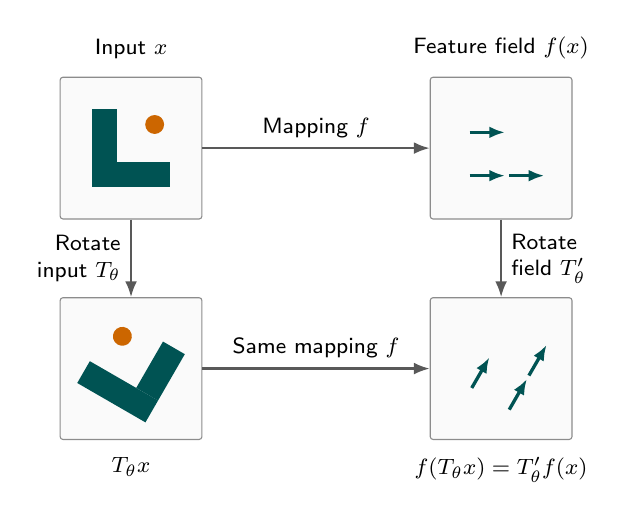
\begin{tikzpicture}[font=\sffamily\footnotesize,
 >={Latex[length=2mm]},flow/.style={->,thick,draw=black!65},
 tile/.style={draw=black!45,rounded corners=1pt,minimum width=18mm,
 minimum height=18mm,fill=black!2,inner sep=0}]
\node[tile] (x) at (0,0) {};
\node[tile] (fx) at (4.7,0) {};
\node[tile] (rx) at (0,-2.8) {};
\node[tile] (rfx) at (4.7,-2.8) {};
\foreach \n/\a in {x/0,rx/60}{
 \begin{scope}[shift={(\n.center)},rotate=\a]
 \fill[teal!65!black] (-.5,-.5) rectangle (-.18,.5);
 \fill[teal!65!black] (-.18,-.5) rectangle (.5,-.18);
 \fill[orange!80!black] (.3,.3) circle[radius=.12];
 \end{scope}
}
\foreach \n/\a in {fx/0,rfx/60}{
 \begin{scope}[shift={(\n.center)},rotate=\a]
 \foreach \p in {(-.4,-.35),(-.4,.2),(.1,-.35)}{
 \draw[->,very thick,teal!65!black] \p -- ++(.45,0);
 }
 \end{scope}
}
\node[above=1mm of x] {Input $x$};
\node[above=1mm of fx] {Feature field $f(x)$};
\node[below=1mm of rx] {$T_\theta x$};
\node[below=1mm of rfx] {$f(T_\theta x)=T'_\theta f(x)$};
\draw[flow] (x.east) -- node[above] {Mapping $f$} (fx.west);
\draw[flow] (rx.east) -- node[above] {Same mapping $f$} (rfx.west);
\draw[flow] (x.south) -- node[left,align=right] {Rotate\\input $T_\theta$} (rx.north);
\draw[flow] (fx.south) -- node[right,align=left] {Rotate\\field $T'_\theta$} (rfx.north);
\end{tikzpicture}
\caption{Rotation equivariance as a transformation law. The two paths from $x$ to the lower-right field agree for an equivariant mapping $f$. The input rotation $T_\theta$ acts on the image; the corresponding output action $T'_\theta$ also rotates vector components when the output contains vector fields. Shapes and arrows are schematic rather than measured VAE features.}
\label{fig:rotation-equivariance}
\end{figure}

\subsection{Multi-Instance Learning}

Whole-slide images can contain billions of pixels. Their size makes processing at native resolution in a single forward pass computationally impractical. A common approach therefore divides each WSI into patches, learns a local representation, and aggregates patch features for slide-level prediction. Attention-based multiple instance learning (MIL) provides a related supervised formulation in which a WSI is treated as a bag of instances and only the bag label is required \cite{ilse_attention_2018}. CLAM combines attention pooling with instance-level clustering \cite{lu_data_2021}. DSMIL combines contrastive patch representation learning with dual-stream aggregation \cite{li_dualstream_2021}, whereas TransMIL models relations among patch instances during aggregation \cite{shao_transmil_2021}. Here, MIL tests the frozen patch representations under the same WSI classification protocol. \autoref{fig:mil-concept} illustrates the slide-to-bag formulation.

\begin{figure}[t]
\centering
\resizebox{0.98\linewidth}{!}{%
\begin{tikzpicture}[font=\sffamily\footnotesize,
 >={Latex[length=2.2mm]},flow/.style={->,thick,draw=teal!65!black},
 box/.style={draw=teal!55!black,rounded corners=3pt,align=center,
 fill=teal!5,minimum height=16mm,text width=23mm},
 patch/.style={inner sep=0,draw=violet!55!black,line width=.5pt}]
\node[anchor=west,inner sep=0] (wsi) at (0,0)
 {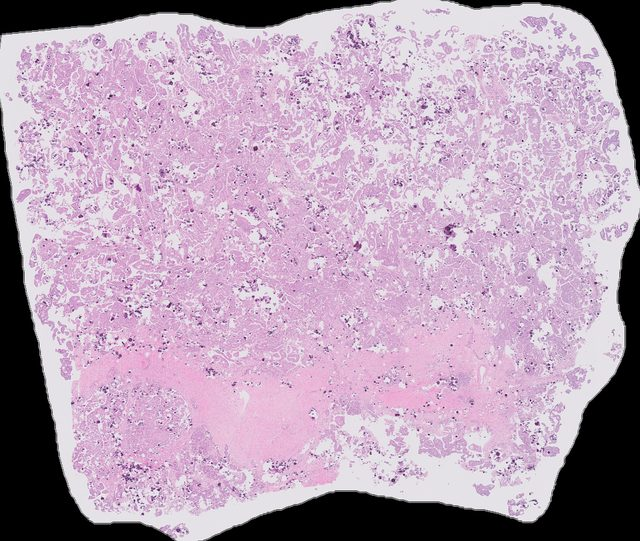
\includegraphics[width=42mm]{figures/mil_11557_thumbnail.jpg}};
\node[below=2mm of wsi,align=center] {Whole-slide image\\\scriptsize WSI thumbnail};
\node[ellipse,draw=violet!55!black,fill=violet!3,line width=.8pt,
 minimum width=52mm,minimum height=49mm,inner sep=0] (bag) at (7.2,0) {};
\node[align=center,font=\sffamily\bfseries\footnotesize] at (7.2,1.9) {Bag of patches};
\foreach \i/\x/\y in {1/6.5/1.1,2/7.8/1.1,3/6.5/0,4/7.8/0,5/6.5/-1.1,6/7.8/-1.1}{
 \node[patch] (p\i) at (\x,\y)
  {\includegraphics[width=9mm]{figures/mil_11557_region_\i.jpg}};
}
\node at (8.65,0) {$\cdots$};
\node[align=center] at (7.2,-1.9) {Thousands of instances};
\foreach \i/\fx/\fy/\py in {
 1/.515625/0.203327/1.55,
 2/.234375/0.277264/.95,
 3/.750000/0.369686/.35,
 4/.531250/0.554529/-.35,
 5/.203125/0.591497/-.95,
 6/.765625/0.702403/-1.55}{
 \coordinate (sx\i) at ($(wsi.north west)!\fx!(wsi.north east)$);
 \coordinate (sy\i) at ($(wsi.north west)!\fy!(wsi.south west)$);
 \coordinate (s\i) at (sx\i |- sy\i);
 \draw[white,line width=1.4pt] ($(s\i)+(-1.5mm,-1.5mm)$) rectangle ++(3mm,3mm);
 \draw[violet!65!black,line width=.65pt] ($(s\i)+(-1.5mm,-1.5mm)$) rectangle ++(3mm,3mm);
 \draw[->,draw=violet!65!black,line width=.65pt]
  (s\i) to[out=0,in=180] (5.25,\py);
}
\node[align=center,text width=22mm] at (4.5,2.05) {Patch\\extraction};
\node[box] (agg) at (12.0,0) {MIL\\aggregation};
\node[box,fill=orange!8,draw=orange!60!black] (pred) at (15.4,0) {Whole-slide\\diagnosis};
\draw[flow] (bag.east) -- node[above,align=center,font=\sffamily\scriptsize]
 {Patch\\features} (agg.west);
\draw[flow] (agg.east) -- (pred.west);
\end{tikzpicture}%
}
\caption{Multiple-instance learning for WSI diagnosis. Many patches extracted from one slide form a bag. Their encoded features are aggregated to predict one whole-slide diagnosis. The six thumbnail regions illustrate the slide-to-bag construction; the ellipsis represents the many remaining instances. In this study, patch features are obtained from frozen VAE posterior means, and supervision is provided by the WSI diagnosis label.}
\label{fig:mil-concept}
\end{figure}


\section{Materials and Methods}
This section describes the UBC-OCEAN dataset, patch selection criteria, and WSI-level data partitions. It then presents the conventional and continuous-$\SOtwo$ denoising VAEs and their training procedure. Finally, it details the evaluation protocols for image reconstruction, patch-level tissue recognition, and WSI-level diagnosis.

\subsection{UBC-OCEAN dataset}

The UBC-OCEAN ovarian-cancer training resource contains 538 slide images: 513 conventional whole-slide images (WSIs) and 25 tissue microarray (TMA) images \cite{ubc_ocean_2023}. A WSI shows a large tissue section; a TMA shows multiple small tissue cores in one image. The resource describes WSIs as large, approximately $20\times$ scans and TMAs as smaller, approximately $4000\times4000$-pixel, $40\times$ images. This scale and layout difference motivated using only the 513 non-TMA WSIs in the present experiment. \autoref{fig:dataset-examples} shows a representative image of each type and their original pixel dimensions. For an image of width $W$ and height $H$, a non-overlapping $256$-pixel grid contains approximately $\lfloor W/256\rfloor\lfloor H/256\rfloor$ full patches before foreground filtering. At the dimensions quoted by the resource, a $4000\times4000$ image yields about 225 full patches, whereas a $100000\times50000$ image yields about 76,000; the latter is an illustrative large-WSI scale, not a count for an individual study slide. The resource also provides $152$ supplemental color masks paired with a subset of those WSIs. These masks mark selected tumor, stroma and necrosis regions; they do not annotate every tissue pixel. The other $361$ WSIs have no supplemental mask. The diagnostic label of each image is one of clear cell carcinoma (CC), endometrioid carcinoma (EC), high-grade serous carcinoma (HGSC), low-grade serous carcinoma (LGSC), or mucinous carcinoma (MC).

Each WSI was divided into non-overlapping RGB $256\times256$-pixel patches. A full WSI has one diagnosis label, so thousands of patches extracted from that slide share the same slide-level label. Local tissue labels, in contrast, come only from eligible regions of the supplemental masks. Splits were made by WSI: no patches from one slide crossed train, validation or test boundaries.

\autoref{fig:dataset-examples} shows two full-resolution patches beside their source WSI thumbnail, a partial supplemental mask on a second WSI, and a TMA. The thumbnail makes the slide-to-patch scale change visible; model inference used crops from the full-resolution WSI. The mask marks selected tissue regions rather than the full image.

\begin{figure}[t]
\centering
\begin{tikzpicture}
    \node[anchor=west,inner sep=0] (slide) at (0,0)
        {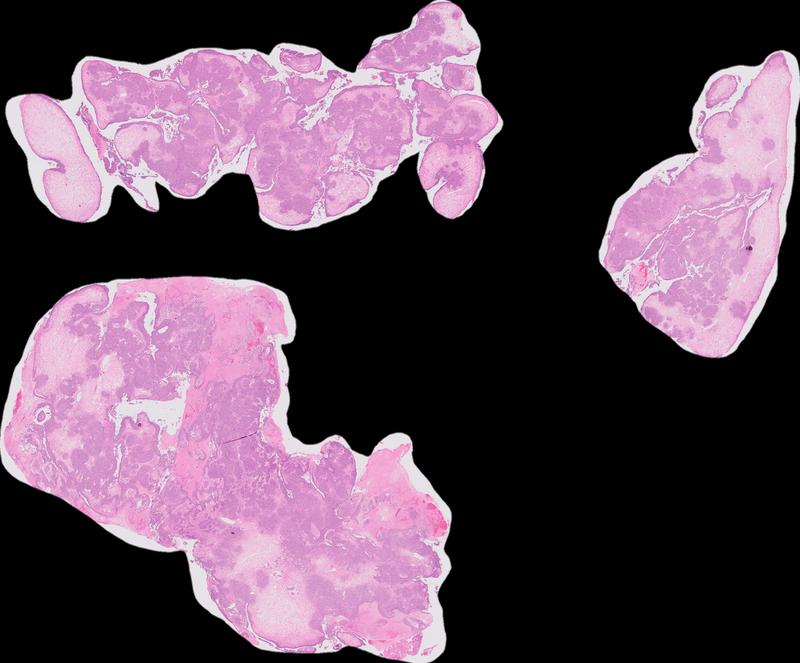
\includegraphics[width=0.52\textwidth]{figures/wsi_59031_thumbnail.jpg}};
    \node[anchor=north west,inner sep=0,draw=blue!70!black,very thick]
        (patchb) at ($(slide.north east)+(1.45cm,0)$)
        {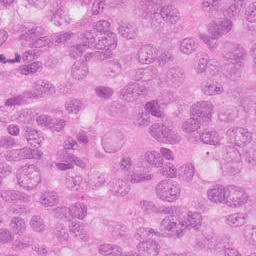
\includegraphics[width=0.17\textwidth]{figures/wsi_59031_patch_13056_4608.png}};
    \node[below=0.7mm of patchb,align=center,text width=0.22\textwidth]
        {\footnotesize (b) Full-resolution patch};
    \node[anchor=south west,inner sep=0,draw=orange!85!black,very thick]
        (patchc) at ($(slide.south east)+(1.45cm,0)$)
        {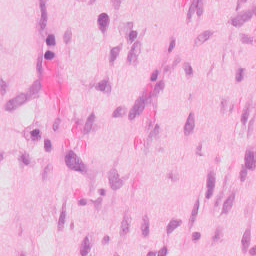
\includegraphics[width=0.17\textwidth]{figures/wsi_59031_patch_44544_9984.png}};
    \node[below=0.7mm of patchc,align=center,text width=0.22\textwidth]
        {\footnotesize (c) Full-resolution patch};

    % Crop centers located on the official 3000x2488 thumbnail by matching
    % downsampled patch pixels: (866,311) and (2933,664), respectively.
    % Horizontal/vertical projections avoid mixing the node's page anchors.
    \coordinate (xb) at ($(slide.north west)!0.288667!(slide.north east)$);
    \coordinate (yb) at ($(slide.north west)!0.125000!(slide.south west)$);
    \coordinate (sourceb) at (xb |- yb);
    \coordinate (xc) at ($(slide.north west)!0.977667!(slide.north east)$);
    \coordinate (yc) at ($(slide.north west)!0.266881!(slide.south west)$);
    \coordinate (sourcec) at (xc |- yc);
    \draw[blue!70!black,very thick,fill=white] (sourceb) circle[radius=1.1mm];
    \node[below right=0.4mm and 0.4mm of sourceb,fill=white,inner sep=1pt,
        text=blue!70!black] {\footnotesize (b)};
    \draw[orange!85!black,very thick,fill=white] (sourcec) circle[radius=1.1mm];
    \node[below left=0.4mm and 0.4mm of sourcec,fill=white,inner sep=1pt,
        text=orange!85!black] {\footnotesize (c)};
    \draw[-{Latex[length=2.2mm]},very thick,blue!70!black]
        (sourceb) to[out=15,in=180] (patchb.west);
    \draw[-{Latex[length=2.2mm]},very thick,orange!85!black]
        (sourcec) to[out=-25,in=180] (patchc.west);
    \node[below=1mm of slide,align=center] {\footnotesize (a) WSI thumbnail};
\end{tikzpicture}
\par\vspace{2mm}
\begin{tabular}{cccc}
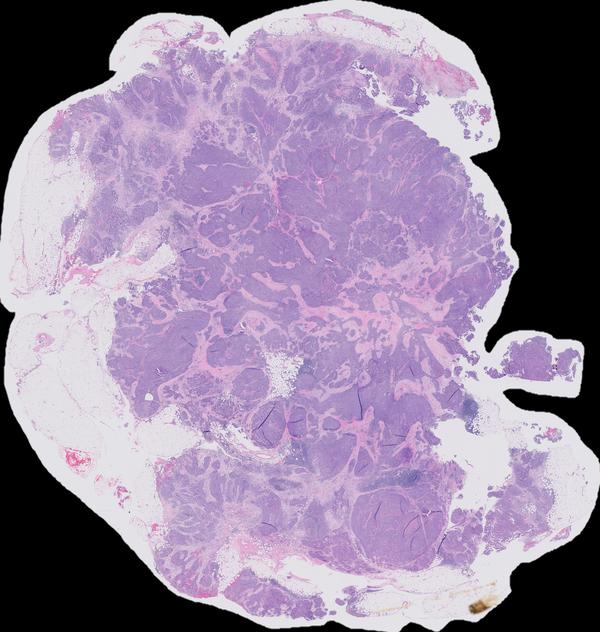
\includegraphics[height=0.115\textheight]{figures/wsi_mask_example_thumbnail.jpg} &
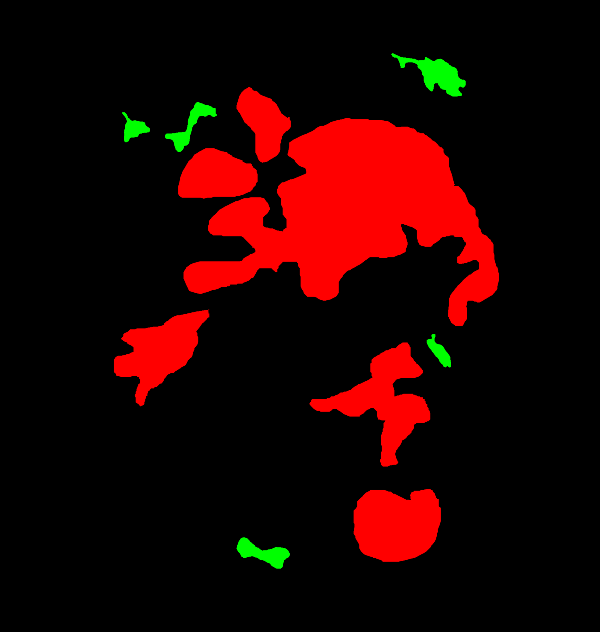
\includegraphics[height=0.115\textheight]{figures/wsi_mask_example_mask.png} &
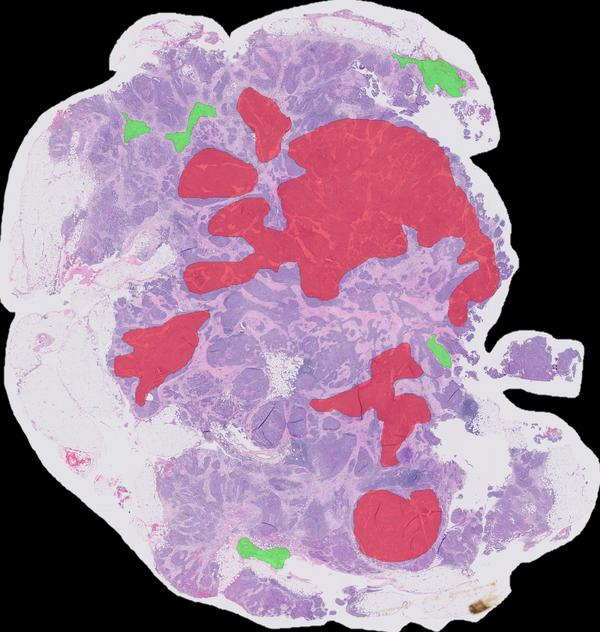
\includegraphics[height=0.115\textheight]{figures/wsi_mask_example_overlay.jpg} &
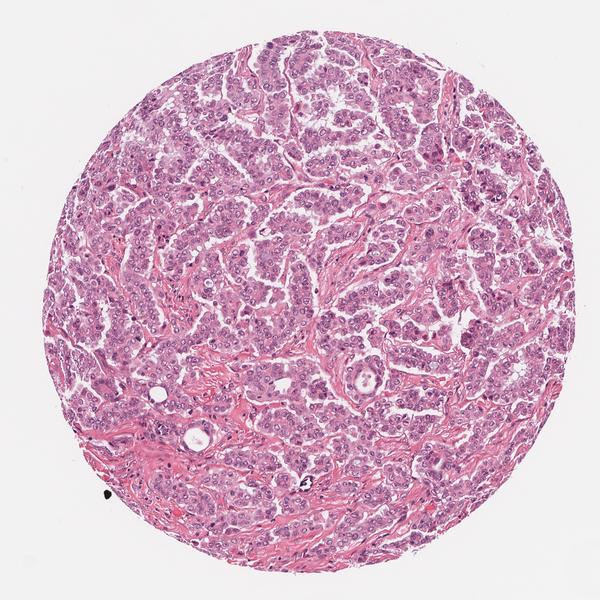
\includegraphics[height=0.115\textheight]{figures/tma_example.jpg} \\
\footnotesize (d) WSI thumbnail &
\footnotesize (e) Partial mask &
\footnotesize (f) Aligned overlay &
\footnotesize (g) TMA
\end{tabular}
\caption{Images and annotations in UBC-OCEAN \cite{ubc_ocean_2023,ubc_ocean_masks_2023}. Panels (a)--(c) show a WSI thumbnail and two actual $256\times256$ crops from that WSI; arrows mark their source regions. Panels (d)--(f) show a different, paired WSI thumbnail, supplemental tissue mask and overlay. Red marks tumor, green stroma and blue necrosis when present; black mask pixels are unannotated. Panel (g) shows a TMA. The WSI in (d) measures $40063\times42207$ pixels, compared with $2964\times2964$ for the TMA. The panels do not share a physical scale; only WSIs enter the experiment.}
\label{fig:dataset-examples}
\end{figure}


% DERB: Revisado hasta acá.  23.10.2026
\subsection{Patch Selection and Tissue Annotations}

Foreground selection for reconstruction and WSI diagnosis was derived from the image rather than from human masks. Each WSI thumbnail was converted to HSV, and Otsu's threshold was applied to the saturation channel \cite{otsu_threshold_1979}. A full-resolution grid cell was retained when more than $60\%$ of its projected thumbnail area belonged to foreground. The resulting coordinates were used for VAE development, reconstruction and WSI diagnosis without consulting the supplemental tissue masks.

Supplemental masks were used only to construct the tissue-recognition population. Red, green and blue mask regions were interpreted as tumor, stroma and necrosis. The masks are not exhaustive; an unpainted region cannot be treated as a negative class. A patch was therefore eligible for tissue classification only when at least $10\%$ of its area was annotated and at least $95\%$ of that annotated area belonged to one tissue class. The resulting task classifies high-purity annotated regions and does not constitute dense pixel-level segmentation of the complete WSI.

\subsection{Data Populations and Partitions}

The 513 eligible WSIs comprise 361 slides for VAE development and a separate cohort of 152 slides with supplemental tissue annotations (\autoref{fig:data-split}). VAE development uses 322 training and 39 validation WSIs, contributing 300,000 and 30,000 unlabeled patches, respectively. Patch sampling supplies 60,000 training and 6,000 validation patches from each WSI diagnosis; diagnosis is not a VAE training target. WSI counts are not balanced by diagnosis (\autoref{tab:task-populations}).

For WSI diagnosis, the same 361-slide development cohort is reused for MIL training and validation through five-fold cross-validation stratified by diagnosis at the WSI level. Fold~0 contains 288 training and 73 validation slides; the remaining four folds contain 289 training and 72 validation slides each. Fold construction also balances the original VAE training or validation role. After cross-validation, a final MIL classifier is trained from scratch for each frozen VAE representation using all 361 development WSIs. The configuration and training duration are fixed based on cross-validation. Final training uses no validation split or validation-based early stopping. Both VAE encoders remain frozen, and the separate 152-WSI cohort is excluded from MIL development and reserved for final evaluation.

For tissue recognition, the 152 annotated WSIs are partitioned into 106 training, 23 validation and 23 test WSIs. Reconstruction evaluation uses the same 23 WSIs as the tissue-recognition test. Assignments are fixed at WSI level and shared by both VAE representations within each task. Diagnosis counts follow the order CC, EC, HGSC, LGSC and MC; tissue counts follow tumor, stroma and necrosis.

For WSI diagnosis, each WSI forms a bag of Otsu-selected foreground patches. Frozen VAE posterior means provide the patch representations, and one diagnosis label supervises the complete bag. The patch-level tissue classifier instead used high-purity annotated tumor, stroma and necrosis patches. Its training subsets were balanced at the five nested label budgets introduced above, whereas validation and test used fixed, unbalanced patch sets. \autoref{tab:task-populations} separates the inputs and class counts of these three stages.

\begin{figure}[p]
\centering
\resizebox{0.98\textwidth}{!}{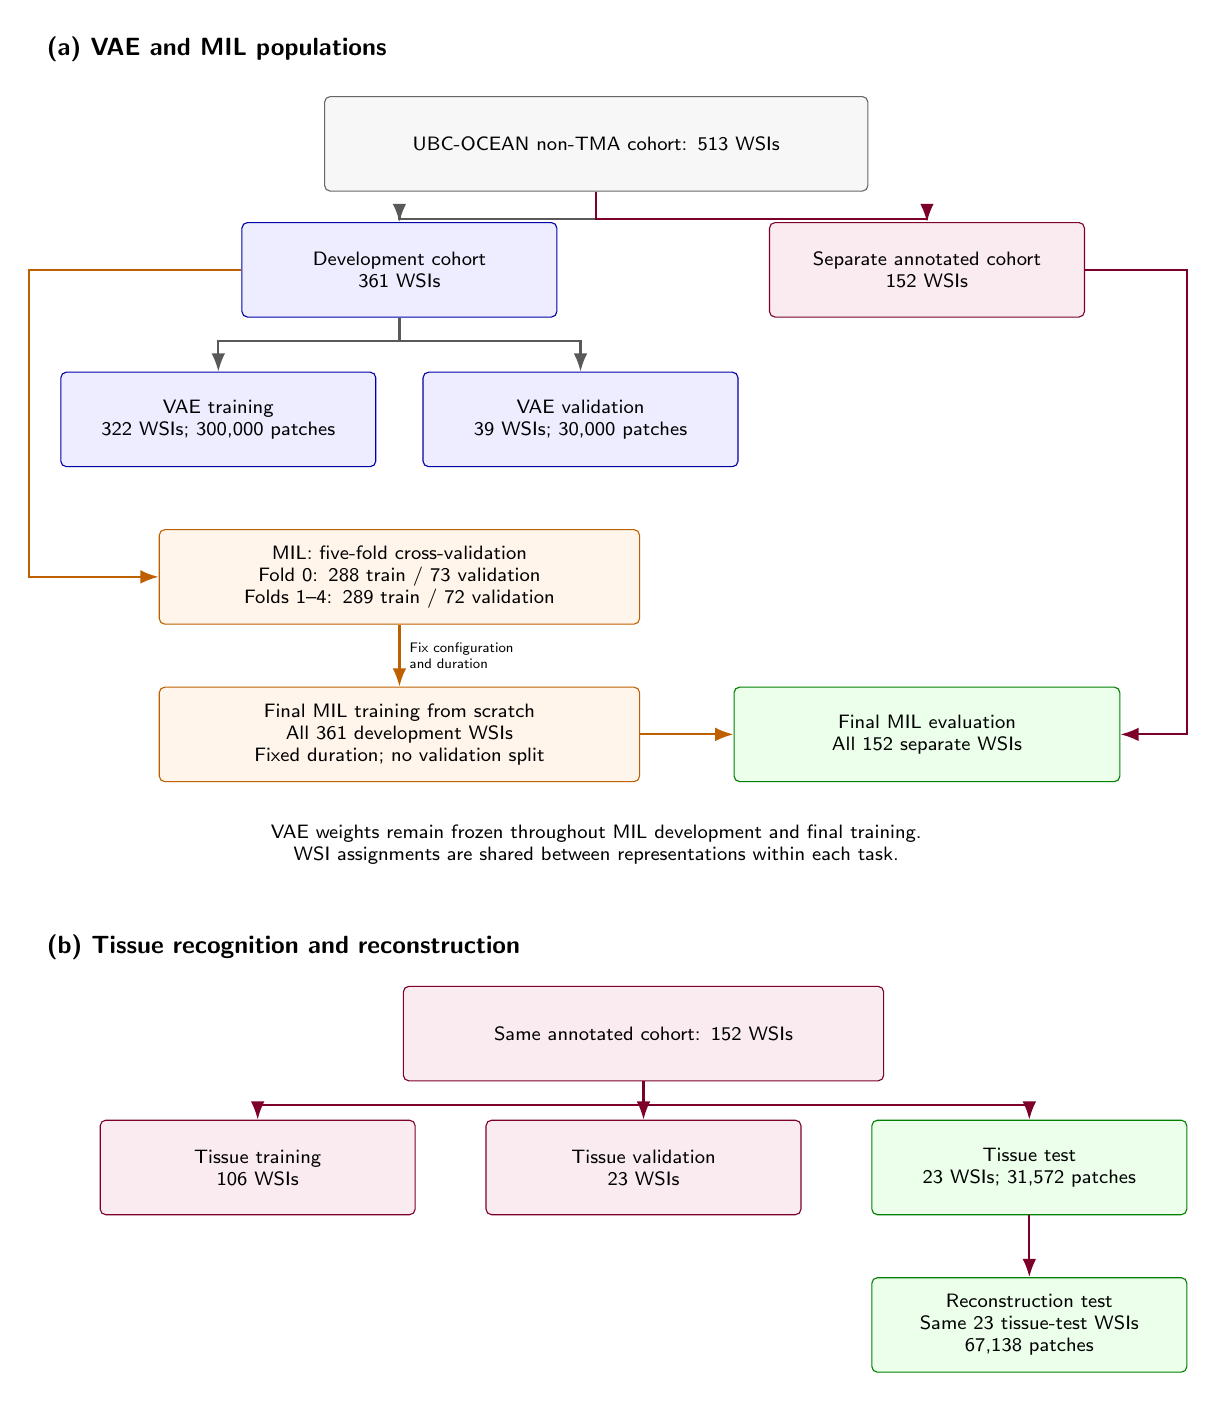
\begin{tikzpicture}[
 font=\sffamily\scriptsize,>=Latex,
 box/.style={draw=black!60,rounded corners=2pt,align=center,text width=36mm,minimum height=12mm,inner sep=2mm},
 vae/.style={box,fill=blue!7,draw=blue!65!black},
 mil/.style={box,fill=orange!8,draw=orange!75!black},
 eval/.style={box,fill=purple!8,draw=purple!65!black},
 task/.style={box,fill=green!8,draw=green!50!black},
 flow/.style={->,thick,draw=black!65},
 milflow/.style={flow,draw=orange!75!black},
 evalflow/.style={flow,draw=purple!65!black}]
\node[box,fill=black!3,text width=65mm] (source) at (4.8,8.0) {UBC-OCEAN non-TMA cohort: 513 WSIs};
\node[vae] (dev) at (2.3,6.4) {Development cohort\\361 WSIs};
\node[eval] (external) at (9.0,6.4) {Separate annotated cohort\\152 WSIs};
\node[vae] (vtrain) at (0,4.5) {VAE training\\322 WSIs; 300,000 patches};
\node[vae] (vval) at (4.6,4.5) {VAE validation\\39 WSIs; 30,000 patches};
\node[mil,text width=57mm] (cv) at (2.3,2.5) {MIL: five-fold cross-validation\\Fold 0: 288 train / 73 validation\\Folds 1--4: 289 train / 72 validation};
\node[mil,text width=57mm] (refit) at (2.3,0.5) {Final MIL training from scratch\\All 361 development WSIs\\Fixed duration; no validation split};
\node[task,text width=45mm] (miltest) at (9.0,0.5) {Final MIL evaluation\\All 152 separate WSIs};
\node[font=\sffamily\bfseries\small,anchor=west] at (-2.3,9.2) {(a) VAE and MIL populations};
\node[font=\sffamily\bfseries\small,anchor=west] at (-2.3,-2.2) {(b) Tissue recognition and reconstruction};
\node[eval,text width=57mm] (annotated) at (5.4,-3.3) {Same annotated cohort: 152 WSIs};
\node[eval] (ttrain) at (0.5,-5.0) {Tissue training\\106 WSIs};
\node[eval] (tval) at (5.4,-5.0) {Tissue validation\\23 WSIs};
\node[task] (ttest) at (10.3,-5.0) {Tissue test\\23 WSIs; 31,572 patches};
\node[task] (recon) at (10.3,-7.0) {Reconstruction test\\Same 23 tissue-test WSIs\\67,138 patches};
\draw[flow] (source.south) -- ++(0,-0.35) -| (dev.north);
\draw[evalflow] (source.south) -- ++(0,-0.35) -| (external.north);
\draw[flow] (dev.south) -- ++(0,-0.3) -| (vtrain.north);
\draw[flow] (dev.south) -- ++(0,-0.3) -| (vval.north);
\draw[milflow] (dev.west) -- ++(-2.7,0) |- (cv.west);
\draw[milflow] (cv.south) -- node[right,font=\sffamily\tiny,align=left] {Fix configuration\\and duration} (refit.north);
\draw[milflow] (refit.east) -- (miltest.west);
\draw[evalflow] (external.east) -- ++(1.3,0) |- (miltest.east);
\draw[evalflow] (annotated.south) -- ++(0,-0.3) -| (ttrain.north);
\draw[evalflow] (annotated.south) -- (tval.north);
\draw[evalflow] (annotated.south) -- ++(0,-0.3) -| (ttest.north);
\draw[evalflow] (ttest.south) -- (recon.north);
\node[font=\sffamily\scriptsize,align=center,text width=110mm] at (4.8,-0.9) {VAE weights remain frozen throughout MIL development and final training.\\WSI assignments are shared between representations within each task.};
\end{tikzpicture}
}
\caption{Data populations and task-specific WSI-level partitions. The 361-slide VAE-development cohort also supplies five-fold MIL cross-validation and final MIL training on all 361 WSIs with no validation split. The separate 152-slide cohort supplies the final MIL evaluation. Within that annotated cohort, tissue recognition uses 106/23/23 training/validation/test WSIs; reconstruction uses the same 23 test WSIs as tissue recognition. The VAE weights remain frozen throughout classifier development.}
\label{fig:data-split}
\end{figure}

\begin{table}[t]
\caption{Inputs by task and split. Diagnosis order is CC/EC/HGSC/LGSC/MC; tissue order is tumor/stroma/necrosis. VAE patch diagnosis is inherited from the source WSI, not a local tissue label. MIL class counts refer to WSIs; tissue class counts refer to patches. MIL bags contain Otsu-selected foreground instances. Dashes indicate patch totals that depend on the fold or are pending for the 152-slide evaluation.}
\label{tab:task-populations}
\centering
\begin{tabular}{@{}llrr>{\raggedright\arraybackslash}p{0.35\textwidth}@{}}
\toprule
Task & Split & WSIs & Patches & Class composition \\
\midrule
VAE & Train & 322 & 300,000 & 54/74/144/24/26 WSIs; 60,000 patches per diagnosis. \\
 & Validation & 39 & 30,000 & 7/9/17/3/3 WSIs; 6,000 patches per diagnosis. \\
\midrule
Reconstruction & Test & 23 & 67,138 & Foreground patches; uncertainty aggregated by WSI. \\
\midrule
Tissue & Train & 106 & 750--17,013 & 250--5,671 selected patches per tissue class. \\
 & Validation & 23 & 31,339 & 22,255/7,809/1,275 patches. \\
 & Test & 23 & 31,572 & 21,796/8,500/1,276 patches. \\
\midrule
WSI MIL & CV train & 288--289 & \textemdash & Four folds; class counts depend on the held-out fold. \\
 & CV validation & 72--73 & \textemdash & One fold; each development WSI is held out once. \\
 & Final train & 361 & 3,056,833 & 61/83/161/27/29 WSI labels; no validation split. \\
 & Final test & 152 & \textemdash & 33/36/56/15/12 WSI labels; separate evaluation cohort. \\
\bottomrule
\end{tabular}
\end{table}

\subsection{Experimental Design}

The same frozen VAE pair is evaluated in three tasks. First, reconstruction measures whether each encoder--decoder recovers clean, unseen patches. Second, a patch classifier uses frozen latent maps to predict local tissue type at five nested label budgets with fixed validation and test sets. Third, an MIL classifier aggregates patch embeddings to predict one diagnosis per WSI. Its development uses five-fold cross-validation on the 361 VAE-development WSIs, followed by final training on all 361 slides and evaluation on the separate 152-slide cohort.

The VAEs were trained on unlabeled patches and frozen before classification. Reconstruction used each encoder and decoder; classification used only the deterministic posterior mean. Both VAEs received the same ordered patches, normalization, corruption policy, loss, update count and validation schedule. Downstream pairs shared WSI assignments, patch coordinates, classifier initialization, epoch order and model-selection rule. The architectures differ in parameter count and computational cost (\autoref{tab:architectures}).

\subsection{Variational Autoencoders and Shared Architecture}

An autoencoder learns to turn an image into a smaller representation and then reconstruct the image from it. Its \emph{encoder} extracts and compresses visual features, and its \emph{decoder} uses the compressed embedding to reproduce the input. In a VAE, the encoder specifies a distribution over embeddings rather than one fixed code: here a diagonal Gaussian with mean $\boldsymbol{\mu}$ and log-variance $\log\boldsymbol{\sigma}^2$. During training, a latent sample $\mathbf{z}$ is drawn by reparameterization \cite{kingma_auto_encoding_2014}. The distribution is regularized toward a unit Gaussian while the decoder learns image reconstruction. After training, the posterior mean is a deterministic feature map for the classifiers. For reconstruction evaluation, the decoder reconstructs the clean patch from that mean. \autoref{fig:vae-pipeline} shows these paths.

Both models used a four-stage residual encoder informed by ResNet-18 \cite{he_deep_2016}: a stem and two residual blocks at each stage, with $2\times$ fixed anti-aliased downsampling between stages. Their decoder used two residual blocks per stage and reversed the three resolution changes with bilinear upsampling followed by convolution. The spatial sequence was $256\rightarrow128\rightarrow64\rightarrow32$ pixels per side in the encoder and reversed in the decoder. Separate posterior heads produced
\begin{equation}
\boldsymbol{\mu},\log\boldsymbol{\sigma}^{2}
\in\mathbb{R}^{16\times32\times32}.
\end{equation}
The decoder returned a raw three-channel image from a zero-initialized output convolution, without a final $\tanh$. The 16-channel spatial embedding preserves coarse locations within the patch; its $32\times32$ grid is smaller than the original $256\times256$ input. \autoref{tab:architectures} compares the two implementations.

\begin{figure}[t]
\centering
\resizebox{0.96\textwidth}{!}{%
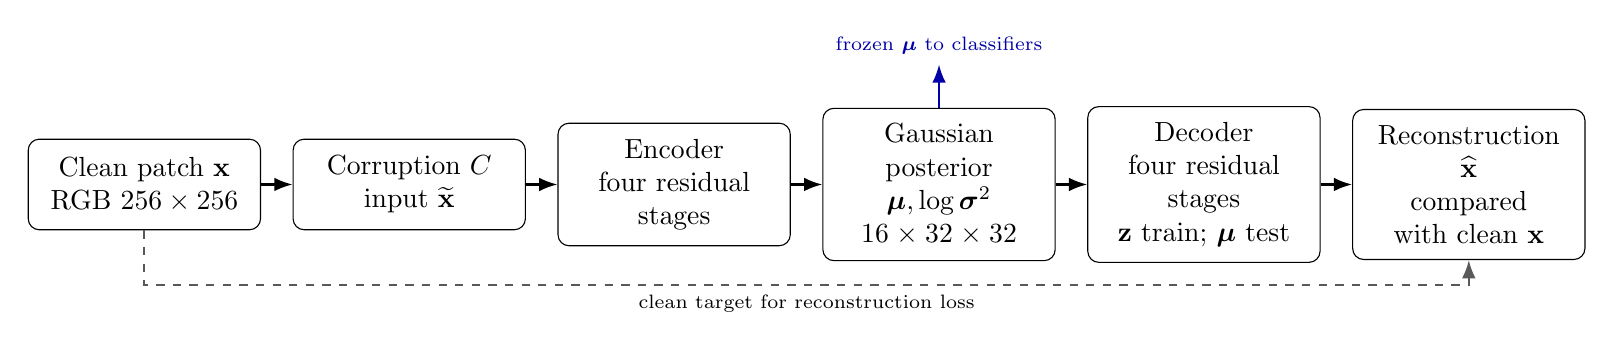
\begin{tikzpicture}[>=Latex, node distance=4mm,
    stage/.style={draw,rounded corners,align=center,minimum height=1.15cm,
                  text width=2.55cm,inner sep=2mm},
    arrow/.style={->,thick}]
\node[stage] (input) {Clean patch $\mathbf{x}$\\RGB $256\times256$};
\node[stage,right=of input] (noise) {Corruption $C$\\input $\widetilde{\mathbf{x}}$};
\node[stage,right=of noise] (encoder) {Encoder\\four residual\\stages};
\node[stage,right=of encoder] (posterior) {Gaussian posterior\\$\boldsymbol{\mu},\log\boldsymbol{\sigma}^2$\\$16\times32\times32$};
\node[stage,right=of posterior] (decoder) {Decoder\\four residual\\stages\\$\mathbf{z}$ train; $\boldsymbol{\mu}$ test};
\node[stage,right=of decoder] (output) {Reconstruction\\$\widehat{\mathbf{x}}$\\compared with clean $\mathbf{x}$};
\draw[arrow] (input)--(noise);
\draw[arrow] (noise)--(encoder);
\draw[arrow] (encoder)--(posterior);
\draw[arrow] (posterior)--(decoder);
\draw[arrow] (decoder)--(output);
\draw[arrow,blue!65!black] (posterior.north) -- ++(0,0.55) node[above,font=\scriptsize] {frozen $\boldsymbol{\mu}$ to classifiers};
\coordinate (targetleft) at (input.south |- {$(posterior.south)+(0,-0.30)$});
\coordinate (targetright) at (output.south |- targetleft);
\draw[arrow,dashed,draw=black!65] (input.south) -- (targetleft) -- (targetright) -- (output.south);
\node[below,font=\scriptsize] at ($(targetleft)!0.5!(targetright)$) {clean target for reconstruction loss};
\end{tikzpicture}%
}
\caption{Shared denoising VAE workflow. Both models have the same input, posterior shape and encoder--decoder resolution schedule. They differ in the type of convolution and the accompanying field normalization and gates. Training reconstructs the clean patch from a possibly corrupted input; classification uses only the frozen posterior mean. The dashed rectangular path supplies the clean input as the reconstruction target.}
\label{fig:vae-pipeline}
\end{figure}

\subsection{Continuous Rotation Equivariance}

A \emph{group} is a collection of transformations that can be composed and inverted. The planar rotation group $\SOtwo$ contains every angle from $0$ to $360$ degrees, with angle addition as its composition rule. A map $f$ is \emph{equivariant} when transforming its input also transforms its output in a predictable way:
\begin{equation}
f(T_g\mathbf{x})=\rho(g)f(\mathbf{x}),\qquad g\in\SOtwo.
\label{eq:equivariance}
\end{equation}
Here $T_g$ rotates an image and $\rho(g)$ specifies how the output feature field must rotate. This is distinct from \emph{invariance}, in which the output stays identical after rotation. For a scalar image feature, spatial locations rotate but the value at a corresponding location does not; for a vector feature, its two components rotate as well.

The conventional VAE used ordinary convolutions, GroupNorm and learned scalar gates. Its hidden channel counts were 32, 48, 64 and 96. The experimental $\SOtwo$ VAE replaced the convolutional layers with steerable convolutions \cite{cohen_steerable_2017,weiler_general_2019}. A steerable kernel is a filter whose rotated version follows a prescribed rule: rather than learning an unrelated filter for every orientation, the network learns coefficients of radial and angular basis functions that obey the input/output field transformation laws. This construction constrains the convolutional operators; it does not by itself establish that the complete trained encoder obeys \autoref{eq:equivariance} exactly under sampled image rotations.

Its hidden features contained $F_0$ scalar fields and $F_1$ vector fields. An $F_0$ copy stores one value per pixel and changes only its spatial location under a rotation. An $F_1$ copy stores an ordered pair of values per pixel; that pair rotates by the same angle as the image coordinate system. Thus, a layout with $n_0$ scalar copies and $n_1$ vector copies has $n_0+2n_1$ numerical channels, not $n_0+n_1$. The four stages used $(n_0,n_1)=(16,16),(24,24),(32,32),(48,48)$. Field-aware normalization and gates based on the $F_1$ vector magnitude were used so these operations respect the field types. The precise nonlinearities and normalizations are given below. The posterior heads returned 16 $F_0$ fields and no $F_1$ fields, matching the conventional $16\times32\times32$ posterior.
\subsubsection{Kernel Support and Learned Parameterization}
\label{sec:kernel-support}
Comparing conventional and rotation-equivariant CNNs is not straightforward: matching kernel support, learned parameter count and computational cost can require different architectural choices. The conventional VAE uses $5\times5$ residual kernels, whereas the $\SOtwo$ VAE uses $7\times7$ steerable kernels. This difference follows from the spatial sampling requirements of the selected steerable basis.

The basis combines angular harmonics with Gaussian radial profiles, a common construction in steerable CNNs \cite{weiler_general_2019}. The radial envelopes are centered at approximately $1.00$, $1.90$ and $2.75$ pixels, each with a standard deviation of $0.30$ pixels. Its $F_1$-to-$F_1$ terms include a second angular harmonic, corresponding to two cycles around the filter center. A centered $5\times5$ grid extends only two pixels along each coordinate axis; only its four corners lie beyond radius $2.5$ pixels. Consequently, the outer radial envelope is sampled unevenly across angles. The $7\times7$ grid extends three pixels along each axis and provides additional samples near this envelope, improving its angular coverage and reducing the risk of discretization aliasing.

While the larger grid might appear to give the steerable layers an advantage, their filters remain constrained to a fixed steerable basis. They learn coefficients of this basis rather than an independent weight at every kernel location. For example, the steerable convolution in the first same-resolution residual stage uses only $30.0\%$ as many learned parameters as its conventional counterpart: 7,680 basis coefficients versus 25,600 free weights. Across the complete VAEs, the $\SOtwo$ model has $29.8\%$ as many learned parameters, although its estimated convolutional work is higher (\autoref{tab:architectures}).

Larger steerable than conventional kernels have also been used in earlier comparisons. Weiler and Cesa used larger steerable kernels to mitigate discretization artifacts while adjusting feature widths to preserve the total parameter count \cite{weiler_general_2019}. Worrall \emph{et al.} compared $5\times5$ harmonic filters with $3\times3$ conventional filters and reported their different parameter counts \cite{worrall_harmonic_2017}. \autoref{fig:residual-blocks} shows the two residual building blocks before \autoref{fig:vae-architectures} assembles them into the full encoder and decoder schedules.

\begin{figure}[t]
\centering
\resizebox{0.98\textwidth}{!}{%
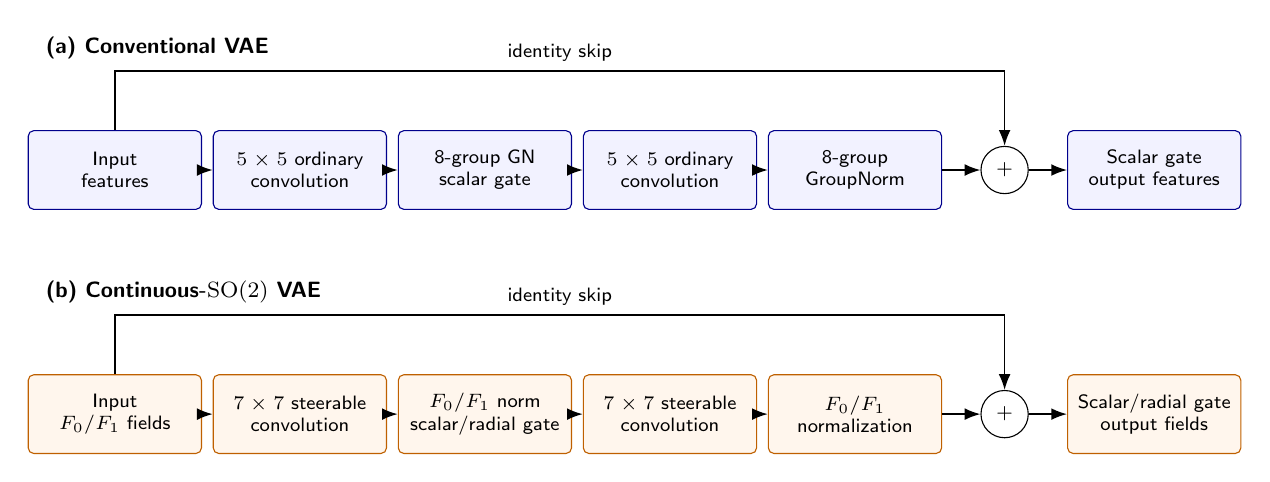
\begin{tikzpicture}[
  font=\sffamily\scriptsize,
  >=Latex,
  box/.style={draw,rounded corners=2pt,align=center,
    minimum height=10mm,text width=20mm,inner sep=1mm},
  flow/.style={-{Latex[length=2mm]},semithick},
  add/.style={draw,circle,minimum size=6mm,inner sep=0pt}
]
\node[anchor=west,font=\sffamily\footnotesize\bfseries] at (-1.0,1.55)
  {(a) Conventional VAE};
\node[box,fill=blue!5,draw=blue!55!black] (a0) at (0,0) {Input\\features};
\node[box,fill=blue!5,draw=blue!55!black] (a1) at (2.35,0) {$5\times5$ ordinary\\convolution};
\node[box,fill=blue!5,draw=blue!55!black] (a2) at (4.7,0) {8-group GN\\scalar gate};
\node[box,fill=blue!5,draw=blue!55!black] (a3) at (7.05,0) {$5\times5$ ordinary\\convolution};
\node[box,fill=blue!5,draw=blue!55!black] (a4) at (9.4,0) {8-group\\GroupNorm};
\node[add] (a5) at (11.3,0) {$+$};
\node[box,fill=blue!5,draw=blue!55!black] (a6) at (13.2,0) {Scalar gate\\output features};
\foreach \from/\to in {a0/a1,a1/a2,a2/a3,a3/a4,a4/a5,a5/a6}
  \draw[flow] (\from)--(\to);
\draw[flow] (a0.north) -- ++(0,0.75) -|
  node[pos=0.25,above] {identity skip} (a5.north);

\node[anchor=west,font=\sffamily\footnotesize\bfseries] at (-1.0,-1.55)
  {(b) Continuous-$\SOtwo$ VAE};
\node[box,fill=orange!7,draw=orange!75!black] (b0) at (0,-3.1) {Input\\$F_0/F_1$ fields};
\node[box,fill=orange!7,draw=orange!75!black] (b1) at (2.35,-3.1) {$7\times7$ steerable\\convolution};
\node[box,fill=orange!7,draw=orange!75!black] (b2) at (4.7,-3.1) {$F_0/F_1$ norm\\scalar/radial gate};
\node[box,fill=orange!7,draw=orange!75!black] (b3) at (7.05,-3.1) {$7\times7$ steerable\\convolution};
\node[box,fill=orange!7,draw=orange!75!black] (b4) at (9.4,-3.1) {$F_0/F_1$\\normalization};
\node[add] (b5) at (11.3,-3.1) {$+$};
\node[box,fill=orange!7,draw=orange!75!black] (b6) at (13.2,-3.1) {Scalar/radial gate\\output fields};
\foreach \from/\to in {b0/b1,b1/b2,b2/b3,b3/b4,b4/b5,b5/b6}
  \draw[flow] (\from)--(\to);
\draw[flow] (b0.north) -- ++(0,0.75) -|
  node[pos=0.25,above] {identity skip} (b5.north);
\end{tikzpicture}%
}

\caption{Same-resolution residual blocks used by the conventional and continuous-$\SOtwo$ VAEs. Each main branch contains two learned convolutions; normalization and a gate follow the first convolution, while the second is followed by normalization. The identity skip is added before the output gate. At encoder stage transitions, both branches are downsampled separately with a fixed $5\times5$ binomial filter: on the main branch after the first gate and on the skip branch before its learned projection and normalization. At decoder transitions, both branches are bilinearly upsampled before their first learned convolution; the skip branch again uses a projection and normalization. The $F_0/F_1$ field types and gate equations are defined in the surrounding text. The $7\times7$ steerable support provides fuller sampling of the selected radial and angular basis; Section~\ref{sec:kernel-support} gives the rationale and learned-parameter comparison.}
\label{fig:residual-blocks}
\end{figure}

\begin{figure}[t]
\centering
\resizebox{0.98\textwidth}{!}{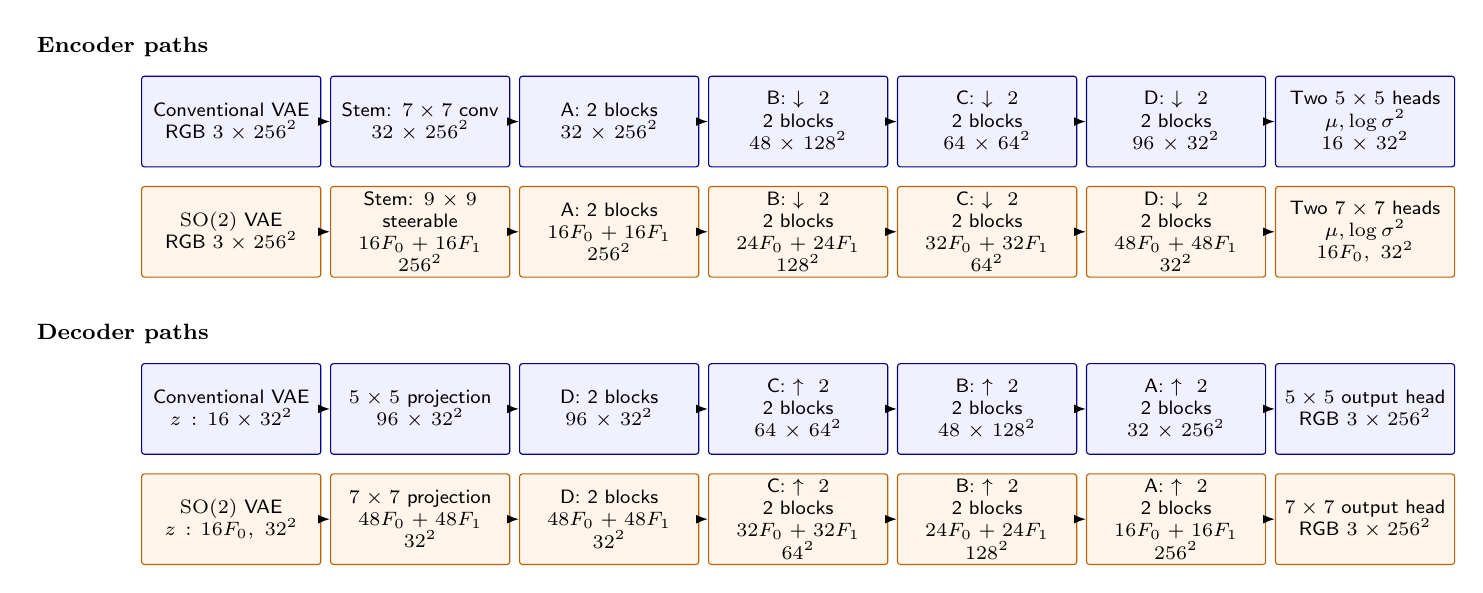
\begin{tikzpicture}[
  x=2.40cm,y=1.25cm,
  stage/.style={draw,rounded corners=1pt,text width=2.17cm,
                minimum height=1.15cm,align=center,inner sep=1.5pt,
                font=\sffamily\scriptsize},
  normal/.style={stage,fill=blue!6,draw=blue!55!black},
  equiv/.style={stage,fill=orange!8,draw=orange!75!black},
  flow/.style={-{Latex[length=1.5mm]},semithick}
]
\node[anchor=west,font=\footnotesize\bfseries] at (-1.08,0.76) {Encoder paths};
\node[anchor=west,font=\footnotesize\bfseries] at (-1.08,-2.16) {Decoder paths};
\node[normal] (ne0) at (0,0) {Conventional VAE\\RGB $3\times256^2$};
\node[normal] (ne1) at (1,0) {Stem: $7\times7$ conv\\$32\times256^2$};
\node[normal] (ne2) at (2,0) {A: 2 blocks\\$32\times256^2$};
\node[normal] (ne3) at (3,0) {B: $\downarrow2$\\2 blocks\\$48\times128^2$};
\node[normal] (ne4) at (4,0) {C: $\downarrow2$\\2 blocks\\$64\times64^2$};
\node[normal] (ne5) at (5,0) {D: $\downarrow2$\\2 blocks\\$96\times32^2$};
\node[normal] (ne6) at (6,0) {Two $5\times5$ heads\\$\mu,\log\sigma^2$\\$16\times32^2$};
\draw[flow] (ne0.east)--(ne1.west);
\draw[flow] (ne1.east)--(ne2.west);
\draw[flow] (ne2.east)--(ne3.west);
\draw[flow] (ne3.east)--(ne4.west);
\draw[flow] (ne4.east)--(ne5.west);
\draw[flow] (ne5.east)--(ne6.west);
\node[equiv] (se0) at (0,-1.12) {$\SOtwo$ VAE\\RGB $3\times256^2$};
\node[equiv] (se1) at (1,-1.12) {Stem: $9\times9$\\steerable\\$16F_0+16F_1$\\$256^2$};
\node[equiv] (se2) at (2,-1.12) {A: 2 blocks\\$16F_0+16F_1$\\$256^2$};
\node[equiv] (se3) at (3,-1.12) {B: $\downarrow2$\\2 blocks\\$24F_0+24F_1$\\$128^2$};
\node[equiv] (se4) at (4,-1.12) {C: $\downarrow2$\\2 blocks\\$32F_0+32F_1$\\$64^2$};
\node[equiv] (se5) at (5,-1.12) {D: $\downarrow2$\\2 blocks\\$48F_0+48F_1$\\$32^2$};
\node[equiv] (se6) at (6,-1.12) {Two $7\times7$ heads\\$\mu,\log\sigma^2$\\$16F_0,\ 32^2$};
\draw[flow] (se0.east)--(se1.west);
\draw[flow] (se1.east)--(se2.west);
\draw[flow] (se2.east)--(se3.west);
\draw[flow] (se3.east)--(se4.west);
\draw[flow] (se4.east)--(se5.west);
\draw[flow] (se5.east)--(se6.west);
\node[normal] (nd0) at (0,-2.92) {Conventional VAE\\$z: 16\times32^2$};
\node[normal] (nd1) at (1,-2.92) {$5\times5$ projection\\$96\times32^2$};
\node[normal] (nd2) at (2,-2.92) {D: 2 blocks\\$96\times32^2$};
\node[normal] (nd3) at (3,-2.92) {C: $\uparrow2$\\2 blocks\\$64\times64^2$};
\node[normal] (nd4) at (4,-2.92) {B: $\uparrow2$\\2 blocks\\$48\times128^2$};
\node[normal] (nd5) at (5,-2.92) {A: $\uparrow2$\\2 blocks\\$32\times256^2$};
\node[normal] (nd6) at (6,-2.92) {$5\times5$ output head\\RGB $3\times256^2$};
\draw[flow] (nd0.east)--(nd1.west);
\draw[flow] (nd1.east)--(nd2.west);
\draw[flow] (nd2.east)--(nd3.west);
\draw[flow] (nd3.east)--(nd4.west);
\draw[flow] (nd4.east)--(nd5.west);
\draw[flow] (nd5.east)--(nd6.west);
\node[equiv] (sd0) at (0,-4.04) {$\SOtwo$ VAE\\$z: 16F_0,\ 32^2$};
\node[equiv] (sd1) at (1,-4.04) {$7\times7$ projection\\$48F_0+48F_1$\\$32^2$};
\node[equiv] (sd2) at (2,-4.04) {D: 2 blocks\\$48F_0+48F_1$\\$32^2$};
\node[equiv] (sd3) at (3,-4.04) {C: $\uparrow2$\\2 blocks\\$32F_0+32F_1$\\$64^2$};
\node[equiv] (sd4) at (4,-4.04) {B: $\uparrow2$\\2 blocks\\$24F_0+24F_1$\\$128^2$};
\node[equiv] (sd5) at (5,-4.04) {A: $\uparrow2$\\2 blocks\\$16F_0+16F_1$\\$256^2$};
\node[equiv] (sd6) at (6,-4.04) {$7\times7$ output head\\RGB $3\times256^2$};
\draw[flow] (sd0.east)--(sd1.west);
\draw[flow] (sd1.east)--(sd2.west);
\draw[flow] (sd2.east)--(sd3.west);
\draw[flow] (sd3.east)--(sd4.west);
\draw[flow] (sd4.east)--(sd5.west);
\draw[flow] (sd5.east)--(sd6.west);
\end{tikzpicture}
}
\caption{Layer-level architecture of the two frozen VAEs. The residual building blocks are detailed in \autoref{fig:residual-blocks}. Each stage A--D contains two residual blocks; stage-changing blocks additionally resample both branches and project the skip branch. A conventional hidden width is a channel count; in the $\SOtwo$ model, $nF_0+nF_1$ means $n$ scalar fields and $n$ two-component vector fields. Posterior mean and log-variance use separate heads; training samples $\mathbf z$, whereas downstream classifiers use $\boldsymbol\mu$. The conventional stem uses a $7\times7$ kernel and its other convolutions use $5\times5$ kernels; the $\SOtwo$ stem uses a $9\times9$ steerable kernel and its other convolutions use $7\times7$ kernels. See Section~\ref{sec:kernel-support} for the kernel-support rationale and learned-parameter comparison.}
\label{fig:vae-architectures}
\end{figure}

\subsection{Field Gates and Normalization}

The conventional VAE applies a learned scalar gate to each hidden channel, including after residual addition. This gate is a parameterized variant of the sigmoid-weighted linear unit (SiLU), $u\,\sigma(u)$ \cite{elfwing_silu_2018}, with a learned slope and offset inside the sigmoid. For a channel value $u_c$,
\begin{equation}
A_0(u_c)=u_c\,\sigma(a_cu_c+b_c),\qquad
\sigma(t)=\frac{1}{1+e^{-t}},
\label{eq:scalar-gate}
\end{equation}
where $a_c$ and $b_c$ are learned per-channel parameters, initialized to $a_c=1$ and $b_c=0$, so the initial activation is SiLU. The $F_0$ fields in the $\SOtwo$ VAE use the same rule with one parameter pair per scalar field. For an $F_1$ field $\mathbf v_j=(v_{j,1},v_{j,2})$, the equivariant VAE gates both components by the same factor computed from their rotation-invariant magnitude:
\begin{equation}
\begin{aligned}
r_j&=\sqrt{v_{j,1}^{2}+v_{j,2}^{2}+10^{-4}},\\
A_1(\mathbf v_j)&=\mathbf v_j\,\sigma(\alpha_j r_j+\beta_j).
\end{aligned}
\label{eq:radial-gate}
\end{equation}
The learned $\alpha_j,\beta_j$ are shared by the two components. A planar rotation changes the vector direction but not $r_j$, so this gate rotates its output together with the input vector.

Before these gates, the conventional network uses affine GroupNorm with eight groups. For each sample and channel $c$, it computes the mean and variance over the channels in $c$'s group and all spatial positions:
\begin{equation}
N_{\mathrm{GN}}(u_c)=\gamma_c
\frac{u_c-\mu_{G(c)}}{\sqrt{s^2_{G(c)}+10^{-5}}}+\delta_c.
\label{eq:group-norm}
\end{equation}
The equivariant network applies this same eight-group formula only to its $F_0$ scalar fields. Its $F_1$ vectors instead use four groups and a shared root-mean-square denominator for both components:
\begin{equation}
N_1(\mathbf v_j)=\gamma_j
\frac{\mathbf v_j}{\sqrt{
\underset{k\in G(j),\,d\in\{1,2\},\,p}{\operatorname{mean}}
 v_{k,d,p}^{2}+10^{-5}}}.
\label{eq:vector-norm}
\end{equation}
Here $p$ indexes spatial positions within one sample. The vector rule has no mean subtraction or additive bias, because either would introduce a preferred direction. Its denominator is unchanged by rotations in feature space. The normalization statistics and gates are evaluated in FP32 in the $\SOtwo$ implementation.

\begin{table}[t]
\caption{Architecture comparison.}
\label{tab:architectures}
\centering
\begin{tabular}{>{\raggedright\arraybackslash}p{0.25\textwidth}>{\raggedright\arraybackslash}p{0.32\textwidth}>{\raggedright\arraybackslash}p{0.34\textwidth}}
\toprule
Property & Conventional VAE & Continuous-$\SOtwo$ VAE \\
\midrule
Hidden representation & Ordinary channels: 32, 48, 64, 96 & $(F_0,F_1)$ copies: (16,16), (24,24), (32,32), (48,48); 48, 72, 96, 144 numerical channels \\
Learned convolutions & 43 ordinary convolutions & 43 steerable convolutions \\
Normalization/\allowbreak{}nonlinearity & Eight-group GroupNorm; learned scalar gate & Eight-group $F_0$ GroupNorm; four-group $F_1$ RMS normalization; scalar and radial gates \\
Posterior & $\boldsymbol{\mu},\log\boldsymbol{\sigma}^{2}\in\mathbb{R}^{16\times32\times32}$ & Same spatial Gaussian posterior, represented by scalar fields \\
Learned parameters & 3,958,435 & 1,180,035 \\
Estimated convolutional work & $3.65\times10^{10}$ MAC/sample & $1.598\times10^{11}$ MAC/sample \\
Rotation constraint & None beyond translation-equivariant convolution & Continuous $\SOtwo$ kernel constraint \\
\bottomrule
\end{tabular}
\end{table}

\subsection{VAE Objective and Training}

Both models used a denoising VAE training criterion: an encoder sees a possibly corrupted patch, and the decoder is trained to reconstruct the corresponding clean patch \cite{im_denoising_2017}. In the implemented training procedure, with probability $0.3$ the corruption operator $C$ perturbed hematoxylin/eosin/residual stain coordinates and added image-space Gaussian noise \cite{ruifrok_color_2001}. The resulting input was clamped to the normalized $[-1,1]$ RGB domain. A patch could therefore be clean or corrupted at the input, while its reconstruction target was always the same clean patch:
\begin{equation}
\mathbf{x}\xrightarrow{\ C\ }\widetilde{\mathbf{x}}
\xrightarrow{\ q_{\boldsymbol{\phi}}\ }\mathbf{z}
\xrightarrow{\ D_{\boldsymbol{\theta}}\ }\widehat{\mathbf{x}}
\quad\text{compared with }\mathbf{x}.
\label{eq:denoise-path}
\end{equation}
The encoder distribution $q_{\boldsymbol{\phi}}(\mathbf{z}\mid\widetilde{\mathbf{x}})$ is the diagonal Gaussian determined by the mean and log-variance heads; $D_{\boldsymbol{\theta}}$ is the decoder. During training, $\mathbf{z}=\boldsymbol{\mu}+\boldsymbol{\sigma}\odot\boldsymbol{\epsilon}$, with $\boldsymbol{\epsilon}\sim\mathcal{N}(\mathbf{0},\mathbf{I})$. The implemented loss was
\begin{equation}
\begin{aligned}
\mathcal{L}={}&\operatorname{MAE}(\widehat{\mathbf{x}},\mathbf{x})
+0.1[1-\operatorname{SSIM}(\widehat{\mathbf{x}},\mathbf{x})]\\
&+\beta D_{\mathrm{KL}}\!\left(
q_{\boldsymbol{\phi}}(\mathbf{z}\mid\widetilde{\mathbf{x}})
\,\|\,\mathcal{N}(\mathbf{0},\mathbf{I})\right),
\end{aligned}
\label{eq:vae-loss}
\end{equation}
where MAE measures pixelwise reconstruction error, SSIM measures structural similarity \cite{wang_image_2004}, and the KL term regularizes the input-dependent posterior toward a unit Gaussian. The KL weight increased linearly from zero to $0.01$ during the first 6,000 updates and remained fixed thereafter.

AdamW \cite{loshchilov_adamw_2019} used coefficients $(0.9,0.999)$, $\epsilon=10^{-8}$, weight decay $10^{-5}$ and gradient-norm clipping at $1.0$. The learning rate increased linearly for 600 updates to $10^{-3}$ and then decreased with a cosine schedule to $10^{-5}$. Each model was trained for 60,000 successful updates with a global batch of 50 patches distributed over two NVIDIA T4 GPUs. Validation and checkpointing occurred every 3,000 updates. The comparison used the final update-60,000 checkpoint for both models rather than selecting different VAE checkpoints from the downstream results.

After VAE training, all encoder and decoder parameters were frozen. Downstream tasks used the posterior mean $\boldsymbol{\mu}$ rather than a sampled latent. For every selected coordinate, both encoders received the same RGB patch. The resulting paired latent datasets had identical WSI membership, tissue labels and patch coordinates.

\subsection{Reconstruction Evaluation}

The reconstruction test contained 67,138 foreground patches from the 23 test WSIs. For each slide, eligible foreground coordinates were sorted by row and column ($y$, then $x$). If there were more than 3,000, 3,000 evenly spaced rank positions were selected across that ordered list; otherwise all were retained. Thus, 22 slides contributed 3,000 patches each and one contributed its available 1,138. The cap limited the influence of slides with many more eligible patches. MAE and mean squared error (MSE) were measured in the normalized $[-1,1]$ domain. Peak signal-to-noise ratio (PSNR) and SSIM were measured after conversion to $[0,1]$ and clamping. Mean MAE was the primary reconstruction measure. The other metrics describe complementary error properties.

\subsection{Classification A: Tissue Recognition and Label Budgets}

Tissue classification uses one patch at a time, without combining information across a WSI. It tests how much tissue information each frozen representation retains as the number of labeled training patches changes. The task predicted tumor, stroma or necrosis from a single latent map. The classifier contained three convolutional stages $16\rightarrow32\rightarrow64\rightarrow128$, GroupNorm, GELU activations \cite{hendrycks_gelu_2016}, adaptive average pooling and a linear $128\rightarrow3$ output layer.

Training subsets contained 250, 500, 1,000, 2,500 and 5,671 labeled patches per class. They were class balanced, nested and selected without replacement; every smaller set was a subset of each larger one. WSI-stratified ordering ensured that the smallest subset did not collapse onto a single slide. Each normal/equivariant pair started from identical classifier weights and received the same patch order. Models were optimized for at most 30 epochs, and the best validation macro-F1 checkpoint was retained. The test distribution was not balanced and contained 21,796 tumor, 8,500 stroma and 1,276 necrosis patches from 23 WSIs.

\subsection{Classification B: Five-Class WSI Diagnosis}

The diagnostic task predicts the five ovarian-cancer subtypes. Each Otsu-selected foreground patch is represented by its frozen posterior mean. A trainable patch encoder maps the $16\times32\times32$ latent map to $8\times8$ spatial tokens of width 64 through a $4\times4$, stride-four convolution. Learned spatial embeddings and a residual MLP encode the tokens, and a learned classification token attends to them to produce one patch embedding. Gated attention-based MIL aggregates the patch embeddings through a softmax-weighted sum, followed by a linear five-class prediction layer \cite{ilse_attention_2018}.

The two representation branches share the five WSI-level folds, classifier initialization and WSI order. Training uses AdamW with a class-weighted classification loss; class weights are computed from the training portion of the relevant fold. The current training recipe uses a paired $60\%$ patch subset per WSI presentation, while validation uses complete bags. Each fold checkpoint is selected by minimum mean unweighted validation cross-entropy. Out-of-fold predictions cover all 361 development WSIs once per paired trajectory. Architecture, hyperparameters and the fixed training duration are determined within the development cohort.

Final training starts from a new classifier initialization and uses all 361 development WSIs for each frozen VAE representation. The duration is fixed from cross-validation, with no validation split or validation-based early stopping. Class weights are recomputed from the 361-slide final training cohort. Final evaluation uses complete bags from the separate 152-WSI cohort after all configuration and model-selection decisions are fixed. Macro-F1 is the primary evaluation metric; balanced accuracy, accuracy, mean cross-entropy, classwise F1 and confusion matrices provide secondary summaries.
% TODO: Completar los hiperparametros de la receta MIL final una vez fijados mediante validacion cruzada.

\subsection{Statistical Analysis}

All difference intervals are reported as conventional-minus-equivariant. Reconstruction differences used 10,000 paired cluster-bootstrap replicates at WSI level \cite{field_bootstrapping_2007}. For WSI diagnosis, the primary development summary is macro-F1 computed from the concatenated out-of-fold predictions over the 361 development WSIs. Final-cohort differences use 10,000 paired bootstrap replicates stratified by diagnosis over the 152 evaluation WSIs. Tissue recognition used a paired WSI bootstrap stratified by observed tissue support. The five label-budget macro-F1 differences and the area under the log-budget learning curve (AULC) difference were considered together as six related comparisons. Their $95\%$ intervals were adjusted simultaneously: across the six comparisons, the bootstrap procedure targets $95\%$ coverage for the whole set of differences. A difference interval entirely below zero favors the equivariant model when higher is better; an interval entirely above zero favors the conventional model. An interval containing zero does not establish a statistically significant difference at the $5\%$ level, nor does it establish equivalence. Patch standard deviations describe variation among patches, while confidence intervals resample WSIs as the biological units.

\section{Results}

\subsection{VAE Reconstruction}

\autoref{fig:reconstructions} displays the first nine patches from the fixed set of 25 validation patches. Each original is paired with both frozen models' final reconstruction.

\begin{figure}[t]
\centering
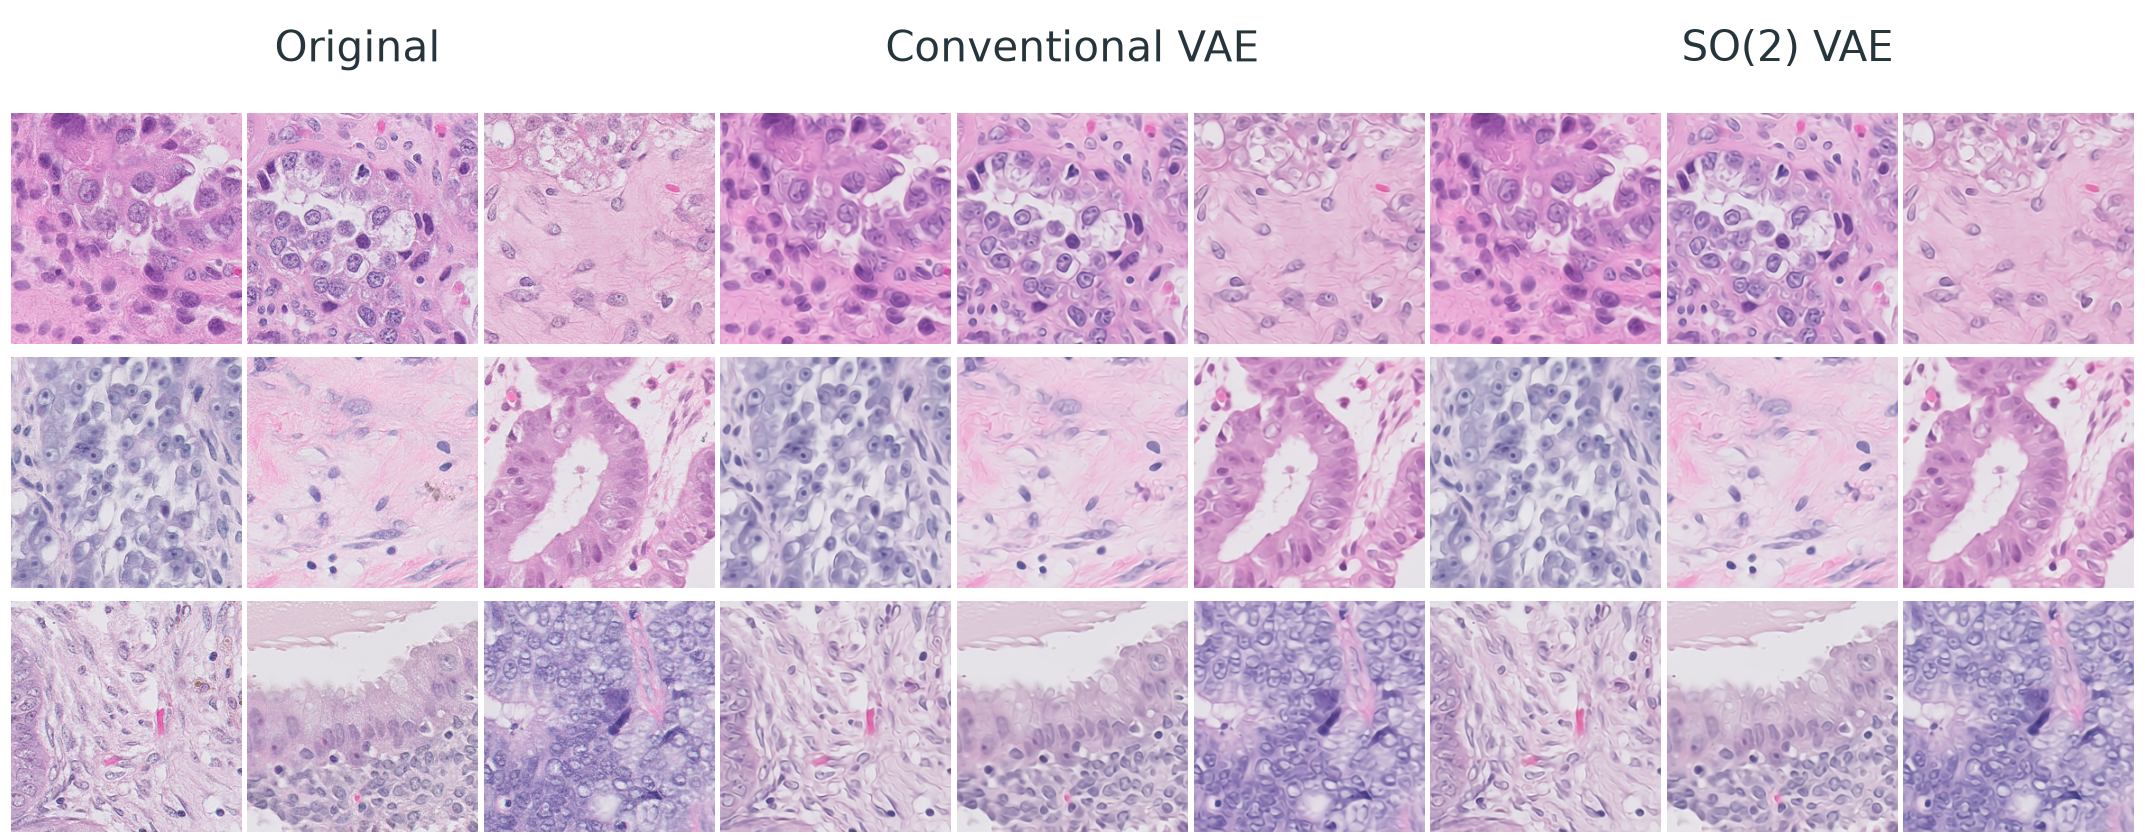
\includegraphics[width=0.96\textwidth]{figures/reconstructions_fixed9.png}
\caption{Three matched $3\times3$ mosaics: original patches, conventional-VAE reconstructions and continuous-$\SOtwo$-VAE reconstructions. The nine examples are the first nine from the fixed set of 25 validation patches; quantitative results use 67,138 patches from 23 test WSIs.}
\label{fig:reconstructions}
\end{figure}

The conventional VAE had lower pooled MAE and MSE and higher pooled PSNR and SSIM (\autoref{tab:reconstruction}). Mean MAE was $0.062872$ for the conventional model and $0.064230$ for the equivariant model. The paired difference was $-0.001358$, with a $95\%$ interval of $[-0.002213,0.000046]$. The interval included zero, so the primary analysis did not establish a reconstruction difference. The remaining metrics are descriptive secondary summaries.

\begin{table}[t]
\caption{Reconstruction on 67,138 test patches. Values are mean (population standard deviation).}
\label{tab:reconstruction}
\centering
\begin{tabular}{lcc}
\toprule
Metric & Conventional & $\SOtwo$ \\
\midrule
MAE $\downarrow$ & $0.0629$ ($0.0239$) & $0.0642$ ($0.0223$) \\
MSE $\downarrow$ & $0.0080$ ($0.0074$) & $0.0083$ ($0.0067$) \\
PSNR dB $\uparrow$ & $27.923$ ($2.721$) & $27.658$ ($2.595$) \\
SSIM $\uparrow$ & $0.7575$ ($0.0842$) & $0.7436$ ($0.0862$) \\
\bottomrule
\end{tabular}
\end{table}

\autoref{fig:reconstruction-boxplots} shows descriptive variation among the 23 test WSIs. Each plotted value is the mean of that WSI's selected test patches; the paired WSI-bootstrap interval above remains the inferential comparison.

\begin{figure}[t]
\centering
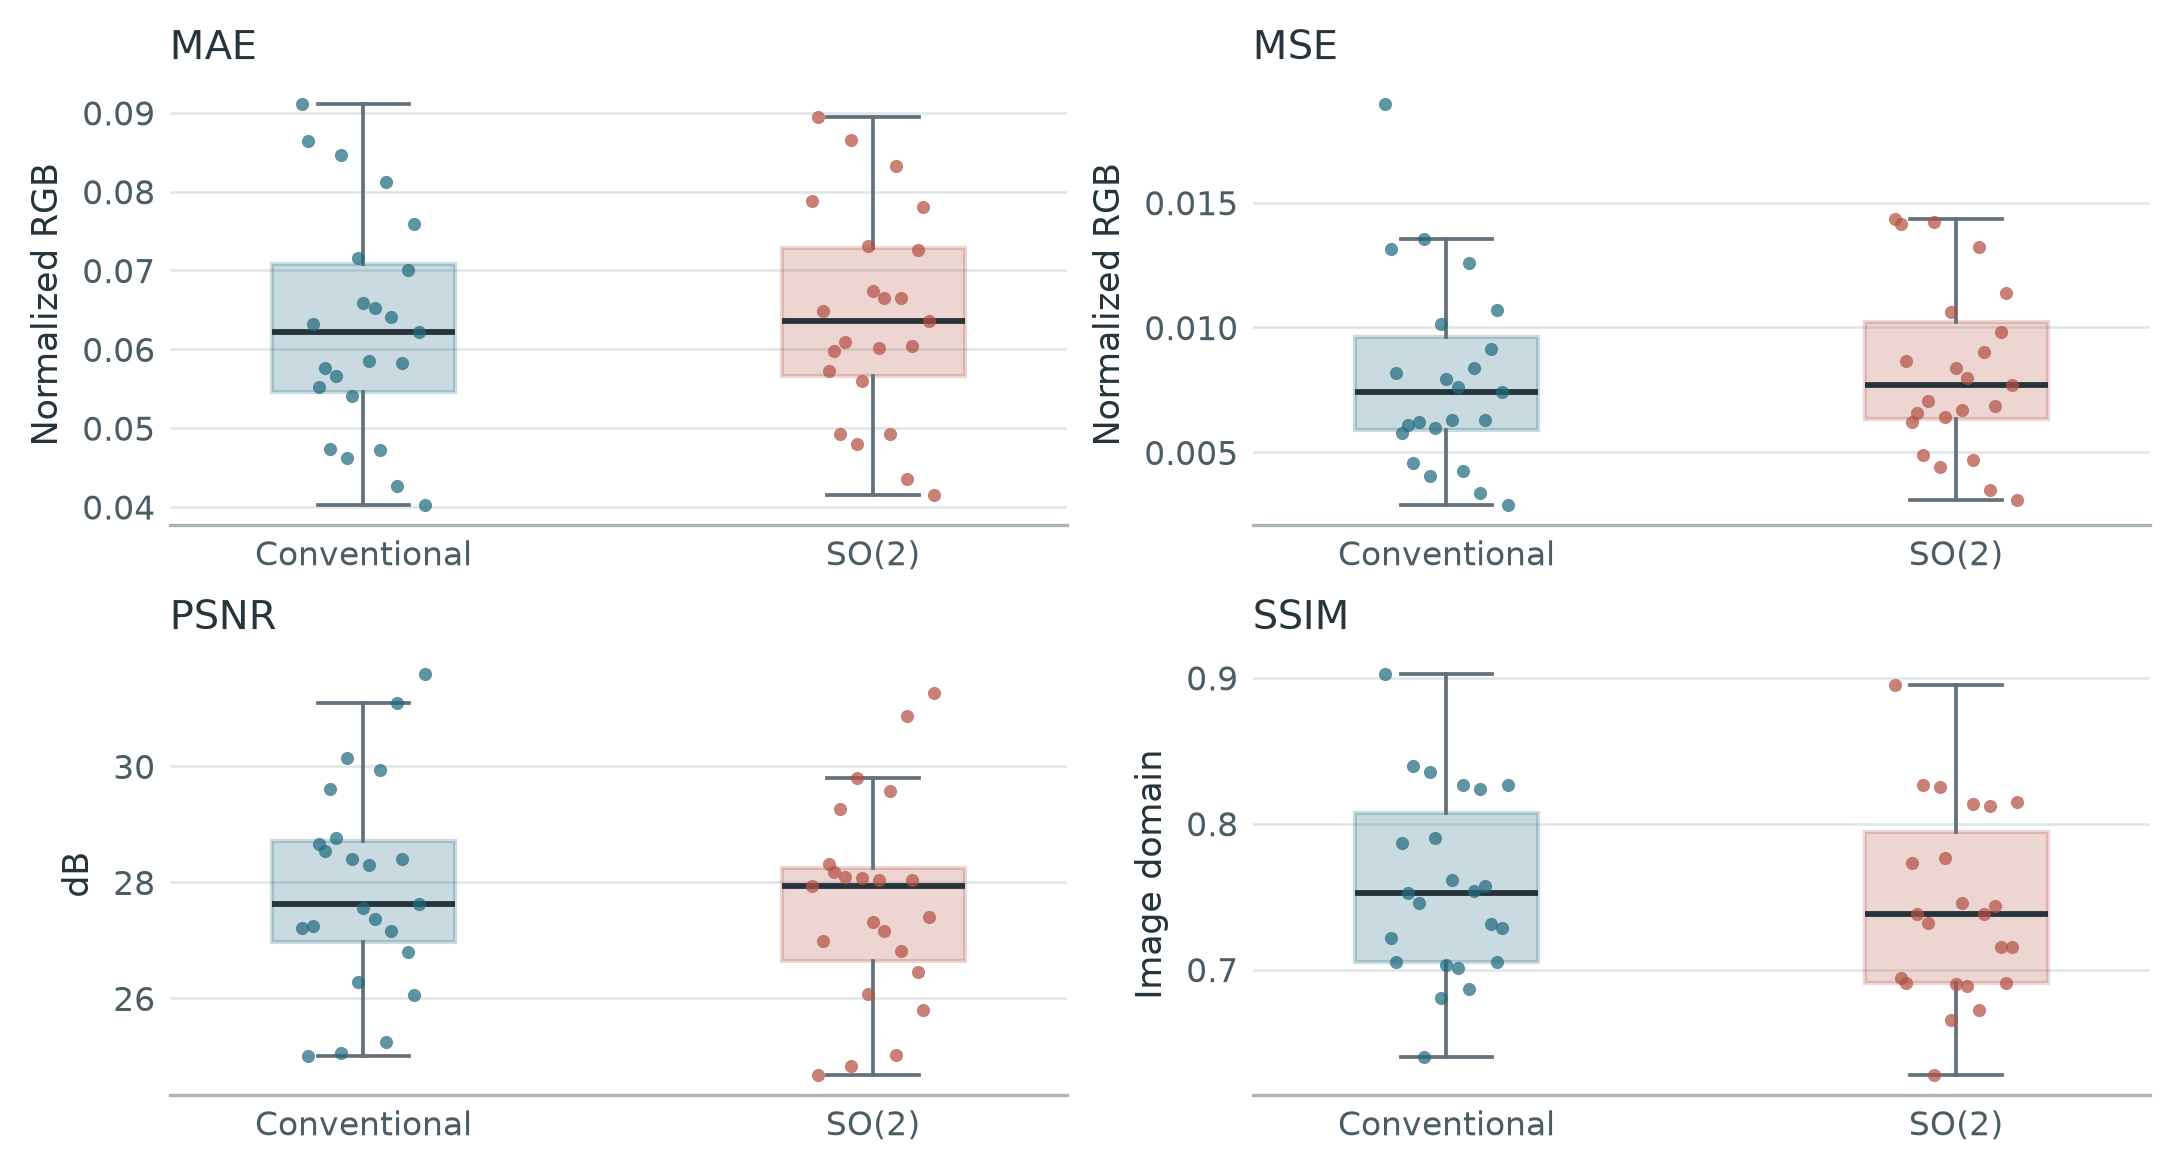
\includegraphics[width=0.88\textwidth]{figures/reconstruction_boxplots.png}
\caption{Reconstruction metric distributions across 23 test WSIs. Each point is one WSI-level mean; boxes summarize those 23 means for each frozen VAE. They are descriptive distributions, not confidence intervals. MAE and MSE use normalized RGB; PSNR and SSIM use image-domain values.}
\label{fig:reconstruction-boxplots}
\end{figure}

\subsection{Classification A: Three-Class Tissue Recognition}

The tissue results changed with the amount of labeled training data (\autoref{fig:downstream} and \autoref{tab:tissue}). The equivariant representation had higher macro-F1 at 250, 500, 1,000 and 2,500 labels per class. At 500 labels per class, the macro-F1 values were $0.575$ and $0.511$, and the simultaneous interval for conventional-minus-equivariant was $[-0.121,-0.008]$. This was the only label budget whose simultaneous interval excluded zero.

At 500 labels per class, the classwise F1 values for conventional/equivariant representations were $0.769/0.781$ for tumor, $0.485/0.560$ for stroma and $0.279/0.384$ for necrosis. These values show how the aggregate macro-F1 difference was distributed across the three tissue classes.

At the largest budget, the conventional representation obtained macro-F1 $0.766$ compared with $0.710$ for the equivariant representation. The simultaneous interval included zero, with a lower bound of $-0.001$. The corresponding classwise F1 values were $0.868/0.871$ for tumor, $0.728/0.711$ for stroma and $0.701/0.548$ for necrosis. The normalized area under the log-budget learning curve was $0.615$ for the conventional representation and $0.631$ for the equivariant representation; its simultaneous difference interval included zero.



\begin{table}[t]
\caption{Tissue macro-F1 on 31,572 test patches. Simultaneous intervals are reported for conventional-minus-$\SOtwo$.}
\label{tab:tissue}
\centering
\begin{tabular}{rccc}
\toprule
Labels/class & Conventional $\uparrow$ & $\SOtwo$ $\uparrow$ & \shortstack{Simultaneous\\$95\%$ CI} \\
\midrule
250 & $0.508$ & $0.523$ & $[-0.072,0.041]$ \\
500 & $0.511$ & $0.575$ & $[-0.121,-0.008]$ \\
1,000 & $0.582$ & $0.598$ & $[-0.072,0.041]$ \\
2,500 & $0.701$ & $0.714$ & $[-0.069,0.044]$ \\
5,671 & $0.766$ & $0.710$ & $[-0.001,0.112]$ \\
\bottomrule
\end{tabular}
\end{table}

\begin{figure}[!t]
\centering
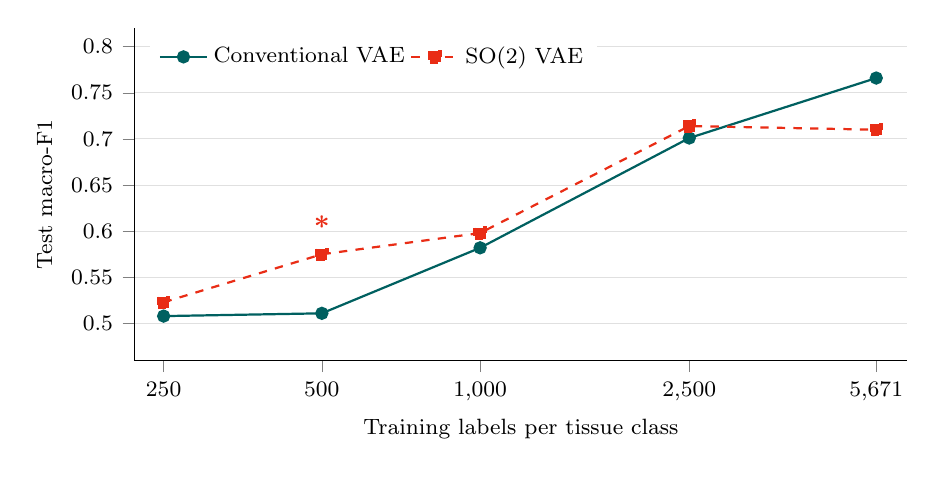
\begin{tikzpicture}
\begin{axis}[
 width=0.94\textwidth,height=5.8cm,
 xmode=log,log basis x=10,xmin=220,xmax=6500,ymin=0.46,ymax=0.82,
 xtick={250,500,1000,2500,5671},xticklabels={250,500,{1,000},{2,500},{5,671}},
 ytick={0.50,0.55,0.60,0.65,0.70,0.75,0.80},
 xlabel={Training labels per tissue class},ylabel={Test macro-F1},
 axis x line*=bottom,axis y line*=left,ymajorgrids=true,
 grid style={draw=black!12},tick align=outside,
 legend style={at={(0.02,0.98)},anchor=north west,draw=none,font=\footnotesize},
 legend columns=2,label style={font=\footnotesize},tick label style={font=\footnotesize}]
\addplot[color=teal!75!black,mark=*,thick] coordinates {(250,0.508) (500,0.511) (1000,0.582) (2500,0.701) (5671,0.766)};
\addlegendentry{Conventional VAE}
\addplot[color=red!65!brown,mark=square*,dashed,thick] coordinates {(250,0.523) (500,0.575) (1000,0.598) (2500,0.714) (5671,0.710)};
\addlegendentry{$\SOtwo$ VAE}
\node[text=red!65!brown,font=\bfseries] at (axis cs:500,0.606) {*};
\end{axis}
\end{tikzpicture}
\caption{Tissue-recognition macro-F1 on 31,572 test patches under nested class-balanced training budgets. The asterisk marks the 500-label contrast whose simultaneous $95\%$ difference interval excludes zero.}
\label{fig:downstream}
\end{figure}

\subsection{Classification B: Five-Class WSI Diagnosis}

The final WSI diagnosis comparison uses the separate cohort of 152 WSIs after five-fold classifier development and final training on all 361 development slides (\autoref{tab:wsi-overall}).
% TODO: Completar las metricas, intervalos y analisis de la evaluacion MIL final de152 WSIs; no trasladar las cifras de23 WSIs.

\begin{table}[t]
\caption{Overall WSI diagnosis results on the separate 152-slide evaluation cohort. Difference intervals are conventional-minus-$\SOtwo$. XXXX/YYYY denote pending final-evaluation values.}
\label{tab:wsi-overall}
\centering
\begin{tabular}{lccc}
\toprule
Metric & Conventional & $\SOtwo$ & Difference $95\%$ CI \\
\midrule
Macro-F1 $\uparrow$ & XXXX & YYYY & \textemdash \\
Balanced accuracy $\uparrow$ & XXXX & YYYY & \textemdash \\
Accuracy $\uparrow$ & XXXX & YYYY & \textemdash \\
Mean cross-entropy $\downarrow$ & XXXX & YYYY & \textemdash \\
\bottomrule
\end{tabular}
\end{table}

The 152-slide evaluation cohort contains 33 CC, 36 EC, 56 HGSC, 15 LGSC and 12 MC WSIs (\autoref{tab:wsi-class}).

\begin{table}[t]
\caption{Classwise WSI F1 and support in the 152-slide evaluation cohort. XXXX/YYYY denote pending final-evaluation values.}
\label{tab:wsi-class}
\centering
\begin{tabular}{lrrr}
\toprule
Diagnosis & Support & Conventional F1 $\uparrow$ & $\SOtwo$ F1 $\uparrow$ \\
\midrule
CC & 33 & XXXX & YYYY \\
EC & 36 & XXXX & YYYY \\
HGSC & 56 & XXXX & YYYY \\
LGSC & 15 & XXXX & YYYY \\
MC & 12 & XXXX & YYYY \\
\bottomrule
\end{tabular}
\end{table}




\section{Discussion}

Which representation scored higher depended on the task and the number of labeled tissue patches. The conventional VAE had lower pooled MAE/MSE and higher pooled PSNR/SSIM point estimates. The equivariant representation had higher tissue macro-F1 at the four smaller budgets. Most confidence intervals for the main comparisons included zero. The single tissue-budget interval that excluded zero applies to that contrast only and does not establish a monotone or general label-efficiency effect. The model with lower reconstruction error did not consistently achieve higher tissue-classification macro-F1.

Patch-based WSI systems depend on both the instance representation and the bag aggregator. Prior MIL work has developed the representation, aggregation or both \cite{ilse_attention_2018,lu_data_2021,li_dualstream_2021,shao_transmil_2021}. The WSI protocol compares the two frozen representations using matched development folds, followed by final training on all 361 development WSIs and evaluation on the separate 152-slide cohort. This design separates classifier development from final evaluation.
% TODO: Completar la discusion WSI con los resultados finales de152 WSIs.

The models also differ in capacity and computation. Graham \emph{et al.} matched parameter counts in comparisons of rotation-equivariant histology classifiers \cite{graham_dense_2020}; these two VAEs were not parameter-matched. The equivariant VAE uses $29.8\%$ as many learned parameters but requires more estimated multiply-accumulate operations. Any performance difference may reflect equivariance, parameter count, optimization or their interaction. The experiment does not separate these mechanisms.

\section{Limitations}


Each VAE and tissue-classification configuration is trained once. The bootstrap intervals quantify variation across the observed WSIs rather than variation across independent VAE training runs. MIL cross-validation estimates classifier performance conditional on fixed representations learned from the same development cohort. The final WSI evaluation contains 152 slides from the same data source. Tissue recognition contains many test patches but only 23 test WSIs, and necrosis is present in five of them.

Supplemental tissue masks are incomplete. The tissue experiment evaluates selected high-purity annotated regions and cannot be interpreted as exhaustive segmentation of complete WSIs. The study uses one ovarian-cancer data source.

\section{Conclusion}

This study compares conventional and continuous-$\SOtwo$ VAEs as frozen histopathology representations under matched task-specific protocols. Reconstruction and tissue-recognition results vary by task and label budget. WSI diagnosis uses five-fold classifier development followed by final training on all 361 development WSIs and evaluation on a separate 152-slide cohort.
% TODO: Completar la conclusion global con la evaluacion MIL final de152 WSIs.

\clearpage
\bibliography{references}

\end{document}
